\documentclass[oneside, openright, titlepage, fleqn, headinclude, 11pt, a4paper, BCOR5mm, footinclude]{scrbook}

%********************************************************************
% Packages
%********************************************************************

\usepackage[utf8]{inputenc}
\usepackage[T1]{fontenc}
\usepackage[italian]{babel}
\usepackage[square, numbers]{natbib}
\usepackage[fleqn]{amsmath}
\usepackage{../packages/dia-classicthesis-ldpkg}
\usepackage[eulerchapternumbers, subfig, beramono, eulermath, parts, subfigure, dottedtoc]{../packages/classicthesis}
\usepackage{xfrac}
\usepackage{marginnote}
\usepackage{placeins}

%********************************************************************
% classicthesis strings
%********************************************************************

\newcommand{\myTitle}{Il Progetto Indico KT\xspace}
\newcommand{\mySubtitle}{Migliorare l'impatto a livello mondiale di Indico\xspace}
\newcommand{\myDegree}{Corso di Laurea Magistrale in Informatica\xspace}
\newcommand{\myName}{Tommaso Papini\xspace}
\newcommand{\myProf}{Pierluigi Crescenzi\xspace}
\newcommand{\mySupervisor}{Pedro Ferreira\xspace}
\newcommand{\myFaculty}{Facoltà di Scienze Matematiche, Fisiche e Naturali\xspace}
\newcommand{\myDepartment}{Dipartimento di Sistemi e Informatica\xspace}
\newcommand{\myUni}{\protect{Università degli Studi di Firenze}\xspace}
\newcommand{\myLocation}{Firenze\xspace}
\newcommand{\myTime}{Anno Accademico 2014-2015\xspace}

%********************************************************************
% Packages options
%********************************************************************

% geometry
\usepackage{geometry}
\geometry{
	a4paper,
	ignoremp,
	bindingoffset = 1cm, 
	textwidth     = 13.5cm,
	textheight    = 21.5cm,
	lmargin       = 3.5cm,
	tmargin       = 4cm
}

% listings
\renewcommand*{\lstlistingname}{Codice}
\newcommand*{\noaddvspace}{\renewcommand*{\addvspace}[1]{}}
\addtocontents{lol}{\protect\noaddvspace}
\let\oldlstlistoflistings\lstlistoflistings
\renewcommand{\lstlistoflistings}{%
    \begingroup%
        \let\oldnumberline\numberline%
        \renewcommand{\numberline}{\!\!\!\!\!\!\!\!\!\lstlistingname~\oldnumberline}%
        \oldlstlistoflistings%
    \endgroup
}
%\lstset{
%    keywordstyle=\color{RoyalBlue},%\bfseries,
%    basicstyle=\small\ttfamily,
%    %identifierstyle=\color{NavyBlue},
%    commentstyle=\color{Green}\ttfamily,
%    stringstyle=\rmfamily,
%    numbers=none,%left,%
%    numberstyle=\scriptsize,%\tiny
%    stepnumber=5,
%    numbersep=8pt,
%    showstringspaces=false,
%    frameround=ftff,
%    frame=single
%    %frame=L
%}
\lstset{
    basicstyle=\small\sffamily,
    numbers=none,
    numberstyle=\tiny,
    numbersep=3pt,
    frame=tb,
    columns=fullflexible,
    backgroundcolor=\color{yellow!20}
}
\lstset{
    numberbychapter=false,
    showstringspaces=false,
    breaklines=true
}

% perpage
\usepackage{perpage}
\MakePerPage{footnote}

% hyperref
\hypersetup{%
    %draft, % = no hyperlinking at all (useful in b/w printouts)
    colorlinks=true, linktocpage=true, pdfstartpage=3, pdfstartview=FitV,%
    % uncomment the following line if you want to have black links (e.g., for printing)
    colorlinks=false, linktocpage=false, pdfstartpage=3, pdfstartview=FitV, pdfborder={0 0 0},%
    breaklinks=true, pdfpagemode=UseNone, pageanchor=true, pdfpagemode=UseOutlines,%
    plainpages=false, bookmarksnumbered, bookmarksopen=true, bookmarksopenlevel=1,%
    hypertexnames=true, pdfhighlight=/O,%nesting=true,%frenchlinks,%
    urlcolor=webbrown, linkcolor=RoyalBlue, citecolor=webgreen, %pagecolor=RoyalBlue,%
    %urlcolor=Black, linkcolor=Black, citecolor=Black, %pagecolor=Black,%
    pdftitle={\myTitle},%
    pdfauthor={\textcopyright\ \myName, \myUni, \myFaculty},%
    pdfsubject={},%
    pdfkeywords={},%
    pdfcreator={pdfLaTeX},%
    pdfproducer={LaTeX with hyperref and classicthesis}%
}

% caption
\captionsetup{format=hang,font=small}

% graphicx
\graphicspath{{img/}}

%********************************************************************
% (Re)new commands & styles
%********************************************************************

% reversed acronym
\newcommand{\acr}[1]{\acs{#1} (\aclu{#1})}

% uppercase part number
\AtBeginDocument{\renewcommand{\thepart}{\Roman{part}}}

% bigger table vertical padding
\setlength{\extrarowheight}{3pt}

% fixed classicthesis chapter number (right-aligned)
\titleformat{\chapter}[display]%
	{\relax}{\mbox{}\oldmarginpar{\vspace*{-3\baselineskip}\makebox[40pt][r]{\color{halfgray}\chapterNumber\thechapter}}}{-5pt}%
	{\raggedright\spacedallcaps}[\normalsize\vspace*{.8\baselineskip}\titlerule]%
	
% language/strings for backrefs
\renewcommand{\backrefnotcitedstring}{\relax}%(Not cited.)
\renewcommand{\backrefcitedsinglestring}[1]{(Citato a pagina~#1.)}
\renewcommand{\backrefcitedmultistring}[1]{(Citato alle pagine~#1.)}
\renewcommand{\backreftwosep}{ e~}
\renewcommand{\backreflastsep}{ e~}

\definecolor{lightgray}{rgb}{.9,.9,.9}
\definecolor{darkgray}{rgb}{.4,.4,.4}
\definecolor{purple}{rgb}{0.65, 0.12, 0.82}
\lstdefinelanguage{javascript}{
  keywords={typeof, new, true, false, catch, function, return, null, catch, switch, var, if, in, while, do, else, case, break},
  keywordstyle=\color{blue}\bfseries,
  ndkeywords={class, export, boolean, throw, implements, import, this},
  ndkeywordstyle=\color{darkgray}\bfseries,
  identifierstyle=\color{black},
  sensitive=false,
  comment=[l]{//},
  morecomment=[s]{/*}{*/},
  commentstyle=\color{purple}\ttfamily,
  stringstyle=\color{red}\ttfamily,
  morestring=[b]',
  morestring=[b]"
}

\definecolor{light-gray}{gray}{0.95}
\newcommand{\bash}[1]{\colorbox{light-gray}{\lstinline[language=bash]{#1}}}
\newcommand{\python}[1]{\colorbox{light-gray}{\lstinline[language=python]{#1}}}
\newcommand{\html}[1]{\colorbox{light-gray}{\lstinline[language=html]{#1}}}
\newcommand{\javascript}[1]{\colorbox{light-gray}{\lstinline[language=javascript]{#1}}}


\begin{document}

    \chapter*{\contentsname}
    
    	\frenchspacing
    	\raggedbottom
    	\pagenumbering{roman}
    	\pagestyle{scrheadings}
    
        \makeatletter
        \documentclass[oneside, openright, titlepage, fleqn, headinclude, 11pt, a4paper, BCOR5mm, footinclude]{scrbook}

%********************************************************************
% Packages
%********************************************************************

\usepackage[utf8]{inputenc}
\usepackage[T1]{fontenc}
\usepackage[italian]{babel}
\usepackage{amsmath}
\usepackage{amssymb}
\usepackage{fancybox}
\usepackage[bottom, para]{footmisc}
\usepackage{graphicx}
\usepackage{hyperref}
\usepackage{packages/mathpartir}
\usepackage{multirow}
\usepackage{pgf}
\usepackage{stmaryrd}
\usepackage{textcomp}
\usepackage{tikz}
\usepackage{titlesec}

%********************************************************************
% Packages options
%********************************************************************

% geometry
\usepackage{geometry}
\geometry{
    a4paper,
    ignoremp,
    bindingoffset = 1cm, 
    textwidth     = 13.5cm,
    textheight    = 21.5cm,
    lmargin       = 1cm,
    rmargin		  = 3cm,
    tmargin       = 2cm,
    bmargin       = 3cm
}

% graphicx
\graphicspath{{img/}}

% tikz
\usetikzlibrary{shapes,shapes.geometric,arrows,fit,calc,positioning,automata}
\tikzset{elliptic state/.style={draw,ellipse}}

%********************************************************************
% New commands
%********************************************************************

\newcommand{\enunciato}[1]{\doublebox{\begin{minipage}{\textwidth}\centering#1\end{minipage}}\\}

\newcommand{\dotxrightarrow}[1]{\;\bullet\!\!\!\xrightarrow{#1}}

\newcommand{\footnoteOP}[1]{
	~\begin{minipage}[b]{4mm}
		~\footnotemark\\
		\(#1\)
	\end{minipage}
}


\begin{document}

	\frenchspacing
	\raggedbottom
	\pagenumbering{roman}
	\pagestyle{plain}
	
%********************************************************************
% Front matter
%********************************************************************

	\begin{center}
   	
\includegraphics[scale=0.5]{logo_title.png}\\[0.8cm]
    {\huge\bfseries Esercizi per l'esame di MSSC}\\
    Anno Accademico 2015/2016\\[0.8cm]

    \begin{tabular*}{\linewidth}{l}
        Tommaso \textsc{Papini}\\
        \href{mailto:tommaso.papini1@stud.unifi.it}{tommaso.papini1@stud.unifi.it}\\
        5537529
    \end{tabular*}\\[1.2cm]
\end{center}

	
	\pagestyle{scrheadings}
	
	\cleardoublepage
\pdfbookmark[1]{Abstract}{Abstract}
\chapter*{Abstract}

	Nel 2014 il \acr{CERN} ha celebrato i suoi \textit{60 anni} di attività.
	
	Dalla sua fondazione, nel lontano Settembre 1954, il \ac{CERN} è stato protagonista di una serie di scoperte e innovazioni in svariati settori scientifici, informatica e fisica in primis, e si è affermato come uno tra i più importanti centri di ricerca in Europa e nel mondo. Il \ac{CERN} è infatti il più grande centro di ricerca di fisica nucleare in Europa, possessore, al momento, del più grande acceleratore di particelle al mondo: l'\acr{LHC}.
	
	Grazie al \ac{CERN} sono state fatte molte scoperte in ambito della fisica delle particelle, come la recente conferma sperimentale dell'effettiva esistenza del tanto cercato \textit{bosone di Higgs}: il 4 Luglio 2012 i team degli esperimenti \acr{ATLAS} e \acr{CMS} confermarono la scoperta del bosone di Higgs, scoperta che portò poi, il 10 Dicembre 2013, al conferimento del premio Nobel per la fisica a Peter Higgs e François Englert, principali ricercatori che teorizzarono l'esistenza di questa particella subatomica.
	
	Ma il \ac{CERN} è stato protagonista anche di molte innovazioni in ambito informatico: pensiamo al servizio internet Web, o \acr{WWW}, che fu ideato proprio al \ac{CERN} nel 1989 da Tim Berners-Lee, adesso fondatore e presidente del \acr{W3C}.
	
	È in questo contesto che si inquadra il progetto \textit{Improving the Worldwide Impact of Indico} che il sottoscritto, Tommaso Papini, ha seguito nel corso dei 14 mesi passati al \ac{CERN} con il programma di \textit{Technical Student} (dal 1 Ottobre 2013 al 30 Novembre 2014), sotto la supervisione di Pedro Ferreira (dipendente del \ac{CERN} ed attuale Project Manager di Indico) al \ac{CERN} e del Prof. Pierluigi Crescenzi (professore presso l'Università degli Studi di Firenze) da Firenze.
	
	Quest'elaborato, volto ad essere un resoconto di questi 14 mesi, sarà suddiviso in tre parti ed esporrà, in modo comprensivo ed esaustivo, il progetto seguito in Indico. All'interno della prima parte verrà esposta una panoramica dell'ambiente \ac{CERN} e del progetto Indico. Nella seconda parte, invece, saranno esposte le varie parti e le varie fasi che hanno composto il progetto stesso nell'arco di questi 14 mesi, assieme ad una panoramica sugli strumenti ed i linguaggi utilizzati. Infine, nella parte conclusiva, si parlerà di altri progetti minori seguiti al \ac{CERN} e si esporranno delle note conclusive del progetto seguito.
	
%	\cleardoublepage

\pdfbookmark[1]{Ringraziamenti}{ringraziamenti}

%\begin{flushright}{\slshape    
%	We have seen that computer programming is an art,\\ 
%	because it applies accumulated knowledge to the world,\\ 
%	because it requires skill and ingenuity, and especially\\
%	because it produces objects of beauty.}\\
%	\medskip --- Donald E. Knuth
%\end{flushright}
%
%\bigskip

\begingroup

	\let\clearpage\relax
	\let\cleardoublepage\relax
	\let\cleardoublepage\relax
	
	\chapter*{Ringraziamenti}
		Ringrazio me stesso, che ho perso tempo a scriverla.

\endgroup
	%********************************************************************
% Table of contents
%********************************************************************

\refstepcounter{dummy}
\pdfbookmark[1]{\contentsname}{tableofcontents}
\setcounter{tocdepth}{2} % <-- 2 includes up to subsections in the ToC
\setcounter{secnumdepth}{3} % <-- 3 numbers up to subsubsections
\manualmark
\markboth{\spacedlowsmallcaps{\contentsname}}{\spacedlowsmallcaps{\contentsname}}
\tableofcontents 
\automark[section]{chapter}
\renewcommand{\chaptermark}[1]{\markboth{\spacedlowsmallcaps{#1}}{\spacedlowsmallcaps{#1}}}
\renewcommand{\sectionmark}[1]{\markright{\thesection\enspace\spacedlowsmallcaps{#1}}}

\clearpage

%********************************************************************
% Other lists
%********************************************************************

\begingroup 
    \let\clearpage\relax
    \let\cleardoublepage\relax
    \let\cleardoublepage\relax

% List of Figures
    \refstepcounter{dummy}
    \pdfbookmark[1]{\listfigurename}{lof}
    \listoffigures

    \vspace*{8ex}

% List of Tables
%    \refstepcounter{dummy}
%    \pdfbookmark[1]{\listtablename}{lot}
%    \listoftables
%        
%    \vspace*{8ex}
    
% List of Listings
    \refstepcounter{dummy}
    \renewcommand*{\lstlistlistingname}{Listato del codice}
    \pdfbookmark[1]{\lstlistlistingname}{lol}
    \lstlistoflistings 

    \vspace*{8ex}
       
% Acronyms
    \refstepcounter{dummy}
    \pdfbookmark[1]{Acronimi}{acronimi}
    \markboth{\spacedlowsmallcaps{Acronimi}}{\spacedlowsmallcaps{Acronimi}}
	\chapter*{Acronimi}
	\begin{acronym}[COMPASS]
    	\acro{ACM}{Association for Computing Machinery}
    	\acro{AD}{Antiproton Decelerator}
    	\acro{ALICE}{A Large Ion Collider Experiment}
    	\acro{API}{Application Programming Interface}
    	\acro{ATLAS}{A Toroidal LHC ApparatuS}
    	\acro{AVC}{AudioVisual and Collaborative Services}
    	\acro{BE}{Beams}
	    \acro{CERN}{Conseil Européen pour la Recherche Nucléaire}
	    \acro{CIS}{Collaboration \& Information Services}
	    \acro{CMS}{Compact Muon Solenoid}
	    \acro{COMPASS}{Common Muon and Proton Apparatus for Structure and Spectroscopy}
	    \acro{CP}{Charge Parity}
	    \acro{CSS}{Cascading Style Sheets}
	    \acro{CSV}{Comma Separated Values}
	    \acro{DB}{Database}
	    \acro{DG}{Director General}
	    \acro{EGEE}{Enabling Grids for E-sciencE}
	    \acro{EN}{Engineering}
	    \acro{FNAL}{Fermi National Accelerator Laboratory}
     	\acro{FP}{Finance, Procurement and Knowledge Transfer}
	    \acro{GS}{General Infrastructure Services}
	    \acro{HEP}{High Energy Physics}
	    \acro{HR}{Human Resources}
	    \acro{HTML}{HyperText Markup Language}
	    \acro{HTTP}{HyperText Transfer Protocol}
	    \acro{IC}{Indefinite Contract}
	    \acro{IHEP}{Institute of High Energy Physics}
	    \acro{IIS}{Internet Information Services}
	    \acro{ILC}{International Linear Collider}
	    \acro{INFN}{Istituto Nazionale di Fisica Nucleare}
	    \acro{IP}{Internet Protocol}
	    \acro{ISOLDE}{On-Line Isotope Mass Separator}
	    \acro{IT}{Information Technology}
	    \acro{JSON}{JavaScript Object Notation}
	    \acro{KT}{Knowledge Transfer}
	    \acro{KVM}{Kernel-based Virtual Machine}
	    \acro{LEAR}{Low Energy Antiproton Ring}
	    \acro{LEIR}{Low Energy Ion Ring}
	    \acro{LEP}{Large Electron–Positron Collider}
	    \acro{LHC}{Large Hadron Collider}
	    \acro{LHCb}{Large Hadron Collider beauty}
	    \acro{LHCf}{Large Hadron Collider forward}
	    \acro{Linac}{Linear Accelerator}
	    \acro{MIME}{Multipurpose Internet Mail Extensions}
	    \acro{MoEDAL}{Monopole and Exotics Detector at the Large Hadron Collider}
	    \acro{OERN}{Organisation Européenne pour la Recherche Nucléaire}
	    \acro{ORDBMS}{Object-Relational Database Management System}
	    \acro{PH}{Physics}
	    \acro{PS}{Proton Synchrotron}
	    \acro{PSB}{Proton Synchrotron Booster}
	    \acro{QEMU}{Quick EMUlator}
	    \acro{REST}{Representational State Transfer}
	    \acro{RHEL}{Red Hat Enterprise Linux}
	    \acro{SL6}{Scientific Linux 6}
	    \acro{SLC6}{Scientific Linux CERN 6}
	    \acro{SMTP}{Simple Mail Transfer Protocol}
	    \acro{SPS}{Super Proton Synchrotron}
	    \acro{SQL}{Structured Query Language}
	    \acro{SSH}{Secure Shell}
	    \acro{SSL}{Secure Sockets Layer}
	    \acro{TE}{Technology}
	    \acro{TOTEM}{TOTal Elastic and diffractive cross section Measurement}
	    \acro{TTY}{Teletypewriter}
	    \acro{UI}{User Interface}
	    \acro{URL}{Uniform Resource Locator}
	    \acro{UUID}{Universally Unique IDentifier}
	    \acro{VM}{Virtual Machine}
	    \acro{W3C}{World Wide Web Consortium}
	    \acro{WSGI}{Web Server Gateway Interface}
	    \acro{WYSIWYG}{What You See Is What You Get}
		\acro{WWW}{World Wide Web}
		\acro{XML}{eXtensible Markup Language}
		\acro{ZODB}{Zope Object Database}
 \end{acronym}
                    
\endgroup

\cleardoublepage
	
%********************************************************************
% Body matter
%********************************************************************
	
	\pagenumbering{arabic}
	
	\part{CERN e Indico}  \label{part:CERN_indico}
		\chapter{CERN} \label{chap:CERN}
	
	Il \ac{CERN}, anche noto come Organizzazione Europea per la Ricerca sul Nucleare, è l'organizzazione che opera il più grande laboratorio di fisica delle particelle al mondo.
	
	Venne istituito il 29 Settembre 1954 da una serie di stati fondatori nei pressi di Ginevra, a cavallo del confine franco-svizzero. Al momento, il CERN vanta un totale di 21 stati membri, dei quali soltanto Israele non europeo.
	
	\begin{figure}[h!]
		\begin{center}
			
\includegraphics[scale=0.1]{cern_logo.jpg}
		\end{center}
		\caption[Logo del CERN]{Logo del CERN.}
		\label{fig:cern_logo}
	\end{figure}
	
	Col termine \ac{CERN} si indica spesso il laboratorio stesso che, al 2013, contava 2\textquotesingle513 membri staff e circa 12\textquotesingle313 tra fellow, collaboratori associati e studenti, rappresentando un totale di 608 università e 113 nazionalità.
	
	L'obiettivo principale del \ac{CERN} è quello di fornire acceleratori di particelle ed altri strumenti e infrastrutture necessarie per le ricerche di fisica delle alte energie.
	
	Al \ac{CERN} è stata anche proposta e sviluppata una prima implementazione del \aclu{WWW}. All'interno del sito di Meyrin del \ac{CERN} è presente il Data Center principale, che vanta una serie di infrastrutture per l'elaborazione di dati, con lo scopo principale di analizzare dati sperimentali provenienti dal complesso degli acceleratori. Per questo motivo, e per il fatto che questi dati dovevano essere disponibili ed analizzabili da molti altri centri di ricerca, spesso molto distanti, il Data Center di Meyrin divenne un grandissimo centro di smistamento dati, formando una vasta rete tra i vari centri di ricerca.
	
	\section{Breve storia} \label{sec:C;storia}
	
		La convenzione che istituì il \ac{CERN} venne ratificata il 29 Settembre 1954 da 12 stati dell'Europa occidentale.
		
		L'acronimo \ac{CERN}, in origine, indicava la sigla francese \emph{\aclu{CERN}} (Consiglio Europeo per la Ricerca sul Nucleare), che rappresentava il consiglio provvisorio istituito nel 1952 dai 12 stati fondatori per la costruzione di un laboratorio di ricerca di fisica nucleare europeo. Quando il consiglio venne sciolto nel 1954 il nome cambiò all'attuale Organizzazione Europea per la Ricerca sul Nucleare (in francese, \emph{\aclu{OERN}}). In quest'occasione si decise di mantenere la vecchia sigla \ac{CERN} al posto della, più brutta e meno d'impatto, sigla \ac{OERN}. Il fisico Heisenberg stesso si pronunciò sul fatto che l'acronimo sarebbe dovuto rimanere \ac{CERN} anche se il nome non lo era più.
		
		Il \ac{CERN} viene considerato un laboratorio di pace in quanto grazie ad esso persone provenienti da tutto il mondo hanno la possibilità di incontrarsi, discutere e collaborare su diversi progetti. Grazie al \ac{CERN} riescono a lavorare assieme anche persone provenienti da stati in guerra tra loro, come ad esempio Israele e Palestina.
		
		Inoltre, il \ac{CERN} venne istituito circa 10 anni dopo la costruzione della bomba atomica come conseguenza principale della II guerra mondiale.
		
		\subsection{Principali scoperte scientifiche} \label{subsec:C;s;principali_scoperte_scientifiche}
		
			In origine, lo scopo principale del \ac{CERN} era quello di studiare i nuclei atomici, ma ben presto l'attenzione si volse verso lo studio della fisica delle alte energie, in particolare all'interazione tra le particelle subatomiche.
			
			\paragraph{1973}Nel 1973 venne scoperta, grazie alla camera a bolle Gargamelle, una particolare interazione tra particelle subatomiche, detta \textit{corrente debole neutra} (Figura \ref{fig:corrente_debole_neutra}) che, nel 1979, permise l'attribuzione del Premio Nobel per la Fisica ad Abdus Salam, Sheldon Glashow e Steven Weinberg, che teorizzarono quest'interazione in passato.
			
			\begin{figure}[h!]
				\begin{center}
					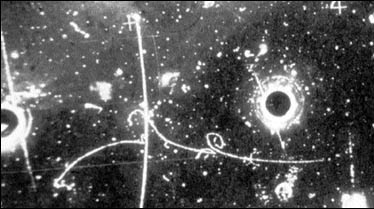
\includegraphics[scale=0.6]{neutral_current.jpg}
				\end{center}
				\caption[Corrente debole neutra]{L'evento di corrente debole neutra osservato con Gargamelle.}
				\label{fig:corrente_debole_neutra}
			\end{figure}
			
			\paragraph{1983}Nel 1983 venne fatta un'altra importantissima scoperta di fisica delle particelle, ovvero la scoperta dei bosoni W e Z. La teorizzazione di questi bosoni fu una conseguenza quasi immediata dell'osservazione della corrente debole neutra, ma prima di poter osservare direttamente queste particelle subatomiche si dovette aspettare di avere un acceleratore di particelle abbastanza potente da produrle. Il primo acceleratore in grado di fare ciò installato al \ac{CERN} fu il \ac{SPS}, che permise, nel Gennaio del 1983 di osservare chiare tracce del bosone W. Gli esperimenti principali furono due, condotti in parallelo, e vennero chiamati UA1 (condotto da Carlo Rubbia) e UA2 (condotto da Pierre Darriulat). I due esperimenti osservarono anche, nel Maggio 1983, i bosoni Z, grazie all'introduzione della tecnica del raffreddamento stocastico introdotta da Simon van der Meer. Nel 1984, la fondazione Nobel, attribuì a Rubbia e Van der Meer il Premio Nobel per la Fisica per l'insostituibile sforzo messo in queste ricerche.
			
			\paragraph{1989}Nel 1989 venne confermato sperimentalmente, utilizzando il \acr{LEP}, che il numero di famiglie di particelle con neutrini leggeri è 3, numero consistente con il Modello Standard.
			
			\begin{figure}[h!]
				\begin{center}
					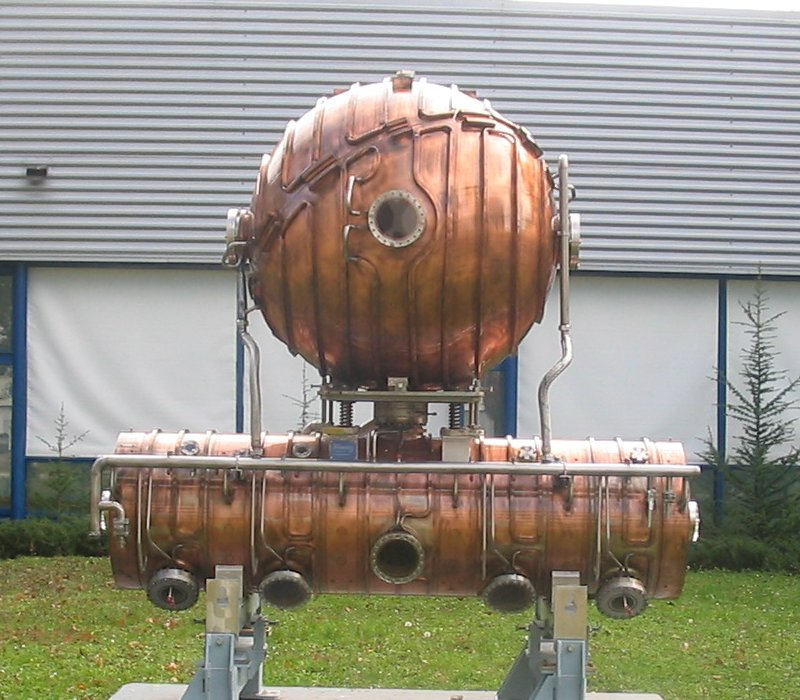
\includegraphics[scale=0.3]{lep_rf.jpg}
				\end{center}
				\caption[Cavità RF del LEP]{Una cavità RF del LEP esposta al Microcosm del CERN.}
				\label{fig:lep_rf}
			\end{figure}
			
			\paragraph{1992}Nel 1992 venne conferito il Premio Nobel per la Fisica a Georges Charpak per ``per l'invenzione e lo sviluppo dei rivelatori di particelle, in particolare della camera proporzionale a multifili''.
			
			\paragraph{1995}Nel 1995 vennero, per la prima volta nella storia, creati atomi di anti-idrogeno grazie all'esperimento PS210 realizzato al \acr{LEAR}. Questi atomi di anti-idrogeno erano molto instabili e si distrussero subito dopo la creazione, ma non senza produrre un segnale elettrico unico, indice che erano effettivamente stati creati atomi di anti-idrogeno.
			
			\paragraph{1999}L'esperimento NA48 dimostrò, nel 1999, la violazione della simmetria \acr{CP}. L'esperimento fu lanciato nel 1990 come successore dell'esperimento NA31 con lo specifico scopo di dimostrare la violazione della simmetria \ac{CP}, la quale afferma che le leggi della fisica dovrebbero rimanere le stesse quando una particella viene sostituita con la sua anti-particella (simmetria di coniugazione di carica, C) e le coordinate spaziali invertite (simmetria di parità, P).
			
			\paragraph{2010}Nel 2010 un gruppo di ricercatori guidati dal fisico Jeffrey Hangst riuscì ad isolare 38 atomi di anti-idrogeno per circa un decimo di secondo, mentre nel 2011 si riuscì a mantenere degli atomi di anti-idrogeno per più di 15 minuti, in modo da poter studiare più a fondo l'antimateria e le sue proprietà.
			
			\paragraph{2012}Infine, nel 2012, venne finalmente osservato un bosone di massa circa $125 \; \sfrac{GeV}{c^2}$ consistente con il tanto cercato bosone di Higgs. Questo bosone venne teorizzato più di 40 anni fa dai ricercatori Peter Higgs e François Englert ed ha una grande importanza per la fisica delle particelle in quanto la sua esistenza può spiegare come mai alcune particelle hanno massa. L'osservazione definitiva del bosone di Higgs avvenne il 4 Luglio 2012, sfruttando le collisioni prodotte dall'\ac{LHC}, e venne osservato in contemporanea dai due esperimenti \ac{CMS} e \ac{ATLAS}. Questa importantissima scoperta portò al conferimento del Premio Nobel per la Fisica, il 10 Dicembre 2013, ai ricercatori Higgs e Englert.
			
		\subsection{Il CERN e l'informatica} \label{subsec:C;s;informatica}
		
			Il primo computer arrivò al \ac{CERN} nel 1959 e da allora i fisici iniziarono ad utilizzare sempre più gli strumenti informatici per le loro analisi. Un elemento importante in questo contesto fu l'italiano Paolo Zanella, capo del dipartimento \acr{IT} per 13 anni, dal 1976 al 1989. Gli esperimenti condotti al \ac{CERN} producevano una mole di dati sempre più grande, tale da rendere impossibile la sola analisi ``a mano''.
			
			Nel tempo, venne anche sperimentato il collegamento fra più calcolatori portando all'utilizzo delle prime reti di calcolatori. Presto, al \ac{CERN} si formò uno dei più grandi centri di calcolo in Europa. Più recentemente si sono iniziate a sviluppare al \ac{CERN} tecnologie per il grid computing, con progetti come \ac{EGEE} o LHC Computing Grid.
			
			\begin{figure}[h!]
				\begin{center}
					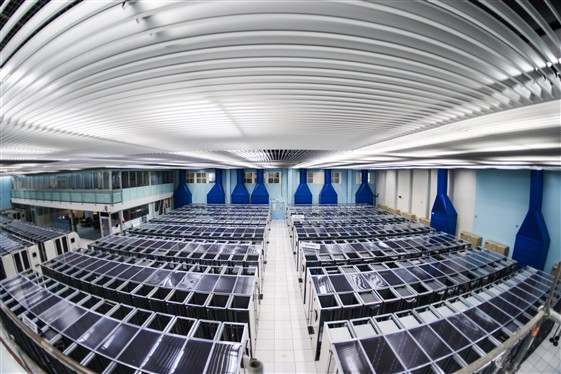
\includegraphics[scale=0.5]{data_center.jpg}
				\end{center}
				\caption[Server Room del Data Center]{L'interno della Server Room del Data Center nel sito di Meyrin.}
				\label{fig:data_center}
			\end{figure}
			
			Il servizio Internet \aclu{WWW} prese vita al \ac{CERN} dal progetto ENQUIRE, condotto da Tim Berners-Lee nel 1989 e Robert Cailliau nel 1990. Nel 1995 Berners-Lee e Cailliau vennero premiati dalla \acr{ACM} per l'indispensabile contributo allo sviluppo del \aclu{WWW}. Il progetto era basato sul concetto di ipertesto, ovvero testo riprodotto su display e collegato ad altri testi tramite iperlink. L'obiettivo originale era quello di facilitare lo scambio di informazioni tra i ricercatori per condurre analisi ed esperimenti.
			
			Il primo sito web fu attivo nel 1991 ed il 30 Aprile 1993 il \ac{CERN} annunciò pubblicamente che il Web sarebbe stato libero per tutti.
			
	\section{Il complesso degli acceleratori} \label{sec:C;acceleratori}
	
		Al \ac{CERN} viene utilizzata una serie di acceleratori, disposti in sequenza in modo da aumentare l'energia delle particelle prima di essere ridirette agli eventuali esperimenti o all'acceleratore successivo. Il logo stesso del \ac{CERN} (Figura \ref{fig:cern_logo}) è ispirato al complesso degli acceleratori presente.
			
		\begin{figure}[h!]
			\begin{center}
				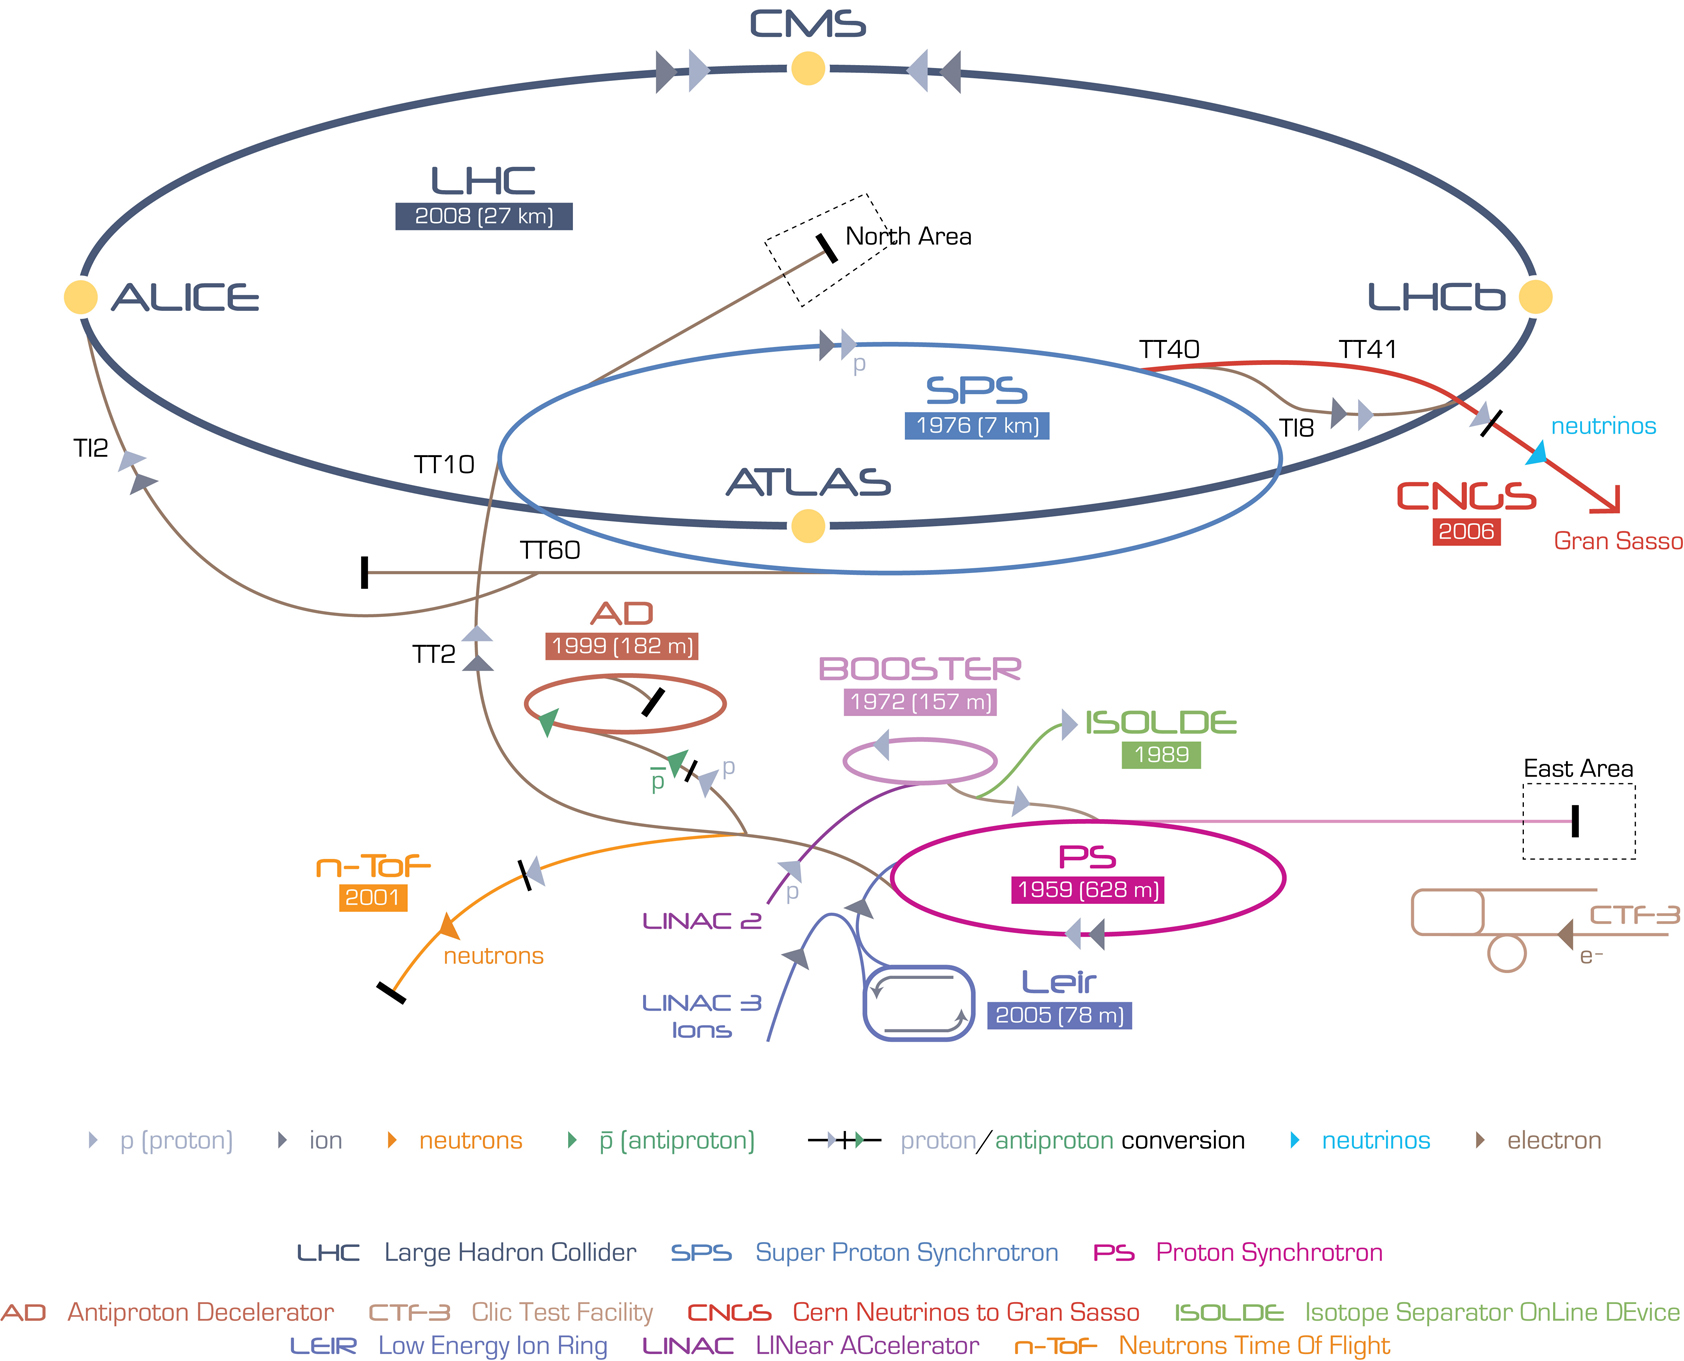
\includegraphics[scale=0.4]{accelerator_complex.jpg}
			\end{center}
			\caption[Complesso degli acceleratori]{Uno schema del complesso degli acceleratori presenti al CERN con legenda.}
			\label{fig:accelerator_complex}
		\end{figure}
		
		I macchinari attualmente attivi al \ac{CERN} sono i seguenti:
		
		\paragraph{Linac2 e Linac3}Questi due acceleratori lineari (\acs{Linac} sta per \aclu{Linac}) generano particelle a bassa energia. Linac2 accelera protoni fino a $50 \; MeV$ per poi iniettarli nel \ac{PSB}, mentre Linac3 genera ioni pesanti a $4.2 \; \sfrac{MeV}{u}$ per iniettarli nel \ac{LEIR}.
		
		\paragraph{Proton Synchrotron Booster}Aumenta l'energia dei protoni prodotti dal Linac2 prima di trasferirli ad altri acceleratori.
		
		\paragraph{Low Energy Ion Ring}Accelera gli ioni pesanti prodotti dal Linac3 prima di trasferirli al \ac{PS}. Questo acceleratore fu commissionato nel 2005 come riconfigurazione del precedente acceleratore, il \ac{LEAR}.
		
		\paragraph{Proton Synchrotron}Accelera le particelle fino a $28 \; GeV$. Fu costruito tra il 1954 ed il 1959 ed è ancora attivo come alimentatore del più potente \ac{SPS}.
		
		\paragraph{Super Proton Synchrotron}Acceleratore circolare installato in un tunnel di 2 Km di diametro ed attivo dal 1976. Fu costruito inizialmente per portare le particelle fino a $300 \; GeV$, per poi essere gradualmente aggiornato fino ai $450 \; GeV$. Questo acceleratore ha i propri esperimenti, al momento \acr{COMPASS} ed NA62, ma veniva anche utilizzato come collisore protoni-antiprotoni e per accelerare elettroni e positroni prima di iniettarli nel \ac{LEP}. Dal 2008 viene invece utilizzato per iniettare protoni e ioni pesanti nell'\ac{LHC}.
		
		\paragraph{On-Line Isotope Mass Separator}Anche indicato con la sigla \acs{ISOLDE}\acused{ISOLDE}, questa struttura viene utilizzata per studiare i nuclei instabili. Ioni radioattivi provenienti dal \ac{PSB} vengono fatti scontrare con un energia tra $1.0$ e $1.4 \; GeV$.
		
		\paragraph{Antiproton Decelerator}Anche noto come \acs{AD}\acused{AD}, serve a ridurre la velocità degli antiprotoni di circa un $10\%$ della velocità della luce per poter studiare l'antimateria.
		
		\paragraph{Compact Linear Collider}Studia la fattibilità di possibili acceleratori lineari futuri.
		
		\subsection{Large Hadron Collider} \label{subsec:C;a;LHC}
			
			L'\ac{LHC} è attualmente il più grande acceleratore di particelle installato al \ac{CERN}, ovvero l'acceleratore principale su cui vengono eseguiti la maggior parte degli esperimenti.
			
			Il tunnel dell'\ac{LHC} è situato 100 metri sotto terra, nella zona tra l'Aeroporto Internazionale di Ginevra e i monti del Giura. Il tunnel ha una circonferenza di circa 27 Km ed era precedentemente occupato dal vecchio acceleratore \ac{LEP}, che venne disattivato definitivamente nel 2000. Gli acceleratori \ac{PS} ed \ac{SPS} vengono utilizzati per pre-accelerare i protoni iniettati nell'\ac{LHC}.
			
			Lungo l'acceleratore sono presenti i suoi sette esperimenti attualmente attivi: \ac{CMS}, \ac{ATLAS}, \acr{LHCb}, \acr{MoEDAL}, \acr{TOTEM}, \acr{LHCf} ed \acr{ALICE}.
			
			\begin{figure}[h!]
				\begin{center}
					\subfloat[][ATLAS]{
						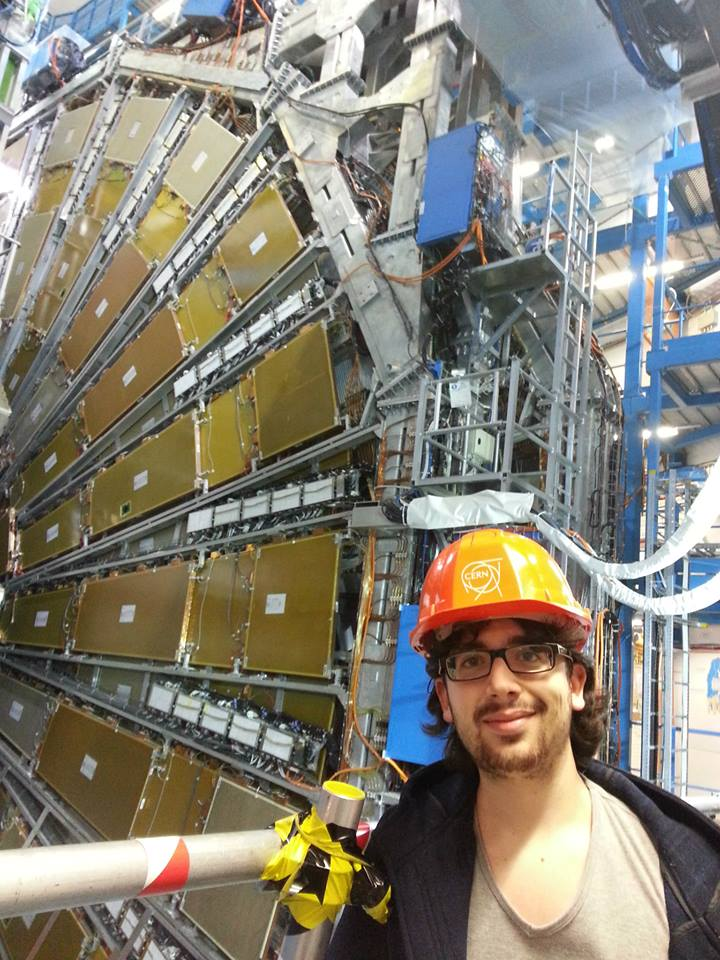
\includegraphics[scale=0.2]{tommaso_atlas.jpg}
					}~
					\subfloat[][CMS]{
						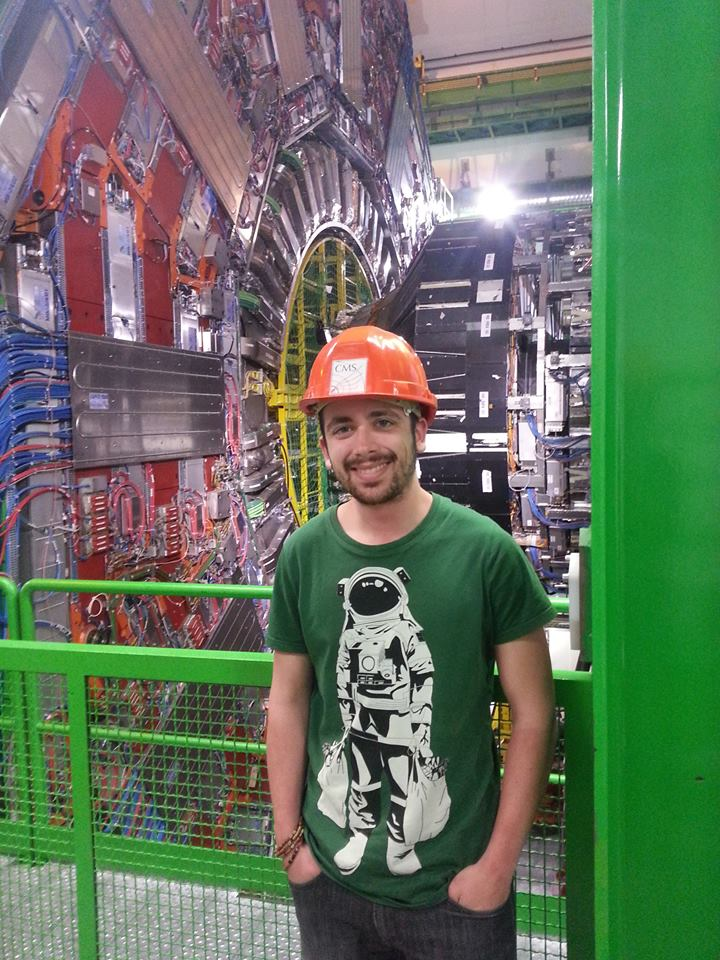
\includegraphics[scale=0.2]{tommaso_cms.jpg}
					}
				\end{center}
				\caption[Visita all'LHC]{Il sottoscritto in visita ad alcuni esperimenti dell'LHC.}
				\label{fig:visita_lhc}
			\end{figure}
			
			L'\ac{LHC} iniziò fin da subito a generare una mole enorme di dati da inviare a diversi laboratori sparsi per il mondo in modo da poter eseguire calcoli distribuiti utilizzando una struttura grid dedicata: la LHC Computing Grid.
			
			Il primo fascio di particelle fu iniettato nell'\ac{LHC} nell'Agosto del 2008 ma, a causa di problemi tecnici, non venne riattivato fino al Novembre del 2009. Il 30 Marzo 2010, invece, si verificò la prima collisione tra due fasci di protoni, ognuno alla velocità di $3.5 \; TeV$, generando una collisione di $7 \; TeV$. Dal Marzo 2012 si passò invece a collisioni di $8 \; TeV$ (ovvero $4 \; TeV$ in ogni direzione). Agli inizi del 2013 l'\ac{LHC} venne disattivato per avviare un periodo di manutenzione e aggiornamento della durata di 2 anni. Dai primi mesi del 2015, l'\ac{LHC} è stato finalmente rimesso in funzione per sperimentare le prime collisioni a $13 \; TeV$. Nel Luglio 2012 venne annunciata l'osservazione sperimentale di una particella subatomica consistente con il tanto agognato bosone di Higgs. Nel Marzo 2013 venne confermato dal \ac{CERN} che, a seguito di una serie di analisi condotte sui dati sperimentali, la particella trovata era effettivamente il bosone di Higgs.
	
	\section{Lavoro al CERN} \label{sec:C;lavoro}
	
		Il \ac{CERN} è il risultato di una collaborazione tra stati, università, scienziati e studenti che sono motivati non da un margine di profitto, ma bensì da un impegno a creare e condividere la conoscenza.
		
		Le persone del \ac{CERN}, sia che siano impiegati fissi, che soltanto di passaggio, prendono parte a ricerche e collaborazioni interessanti con persone di tutto il mondo, cercando di risolvere i misteri della fisica o di creare qualcosa di nuovo.
		
		\subsection{Cultura e valori} \label{subsec:C;l;cultura_e_valori}
		
			Al \ac{CERN} vige il Code of Conduct (Codice della Condotta), ovvero una guida su come trattare gli altri colleghi in accordo con i valori del \ac{CERN}. \cite{cern:culture_values}
			
			I cinque valori di base su cui si basa il \ac{CERN} sono:
			
			\paragraph{Integrit\`{a}}Ovvero comportarsi in modo etico, onesto e ritenersi responsabile delle proprie azioni.
			
			\paragraph{Impegno}Dimostrare, durante il proprio lavoro, un alto livello di motivazione e dedizione verso l'organizzazione ed il proprio progetto.
			
			\paragraph{Professionalit\`{a}}Produrre risultati di alta qualità rispettando i limiti di tempo e le risorse previsti per il completamento del lavoro.
			
			\paragraph{Creativit\`{a}}Promuovere l'innovazione nel proprio settore di lavoro e permettere lo sviluppo e l'evoluzione dell'organizzazione.
			
			\paragraph{Diversit\`{a}}Ovvero saper apprezzare le differenze e promuovere l'uguaglianza e la collaborazione.
		
		\subsection{Carriera al CERN} \label{subsec:C;l;carriera}
		
			Il \ac{CERN} ammette un ampio ventaglio di possibilità per fare carriera ed acquisire esperienza lavorativa al suo interno. Ci sono svariati tipi di contratti per tutti i tipi di aspiranti dipendenti o collaboratori \ac{CERN}: contatti di pochi mesi o contratti di anni, contratti per studenti, per laureati o per professionisti, ecc\dots \cite{cern:carreer}
			
			Uno dei principi di assunzione e lavoro al \ac{CERN} è la non rinnovabilità del contratto: ogni tipo di contratto può essere assegnato ad ogni individuo al più una sola volta. Questo serve a garantire la diversità ed il continuo ricambio di personale ed allo stesso tempo formare abitanti degli stati membri con un'esperienza di alto livello.
			
			\paragraph{Studente}In qualità di studente universitario si hanno molte possibilità di lavoro al \ac{CERN} con contratti di Summer, Admin, Technical e Doctoral Student. Il programma di Technical Student, vissuto dal sottoscritto, prevede una durata dai 6 ai 12 mesi, con la possibilità di estendere il contratto di 2 ulteriori mesi (risorse permettendo). Questi tipi di contratto permettono agli studenti di fare esperienza sul campo ed affrontare sfide intellettuali con alte possibilità di formazione.
			
			\paragraph{Laureato}I contratti per laureati durano normalmente dai 2 ai 3 anni e permettono una formazione ad alto livello. I principali contratti di questo tipo sono la Fellowship, il Graduate Engineer Training ed il contratto Marie-Curie.
			
			\paragraph{Staff}I contratti di Staff durano 5 anni e sono uno dei più ambiti e prestigiosi tipi di contratto al \ac{CERN} come dipendente effettivo e professionista.
			
			\paragraph{E dopo...}Purtroppo anche i contratti di Staff sono non rinnovabili ed a tempo determinato (5 anni). Tuttavia, verso gli ultimi anni di contratto, il \ac{CERN} da la possibilità al membro dello Staff di fare domanda per il cosiddetto \ac{IC}, ovvero un contratto di Staff a tempo indeterminato.
	
		\subsection{La struttura generale} \label{subsec:C;l;struttura}
		
			Il consiglio del \ac{CERN} è la più alta autorità dell'intera organizzazione ed è responsabile di tutte le decisioni più importanti. Si occupa di controllare tutte le attività scientifiche, tecniche ed amministrative del \ac{CERN} e di approvare programmi, attività, budget e spese. Il consiglio è composto da 21 stati membri, ognuno dei quali fornisce due delegati come rappresentanti nel consiglio. Uno dei due delegati rappresenterà gli interessi amministrativi del proprio governo, mentre l'altro rappresenterà gli interessi scientifici nazionali. Nel consiglio, ogni stato membro ha a disposizione un solo voto e per la maggior parte delle decisioni si vota per maggioranza. Il consiglio è assistito, nelle sue decisioni, dalla Scientific Policy Commmittee e dalla Finance Committee.
			
			La Scientific Policy Committee (Commissione della Politica Scientifica) valuta i pro e i contro delle attività proposte dai fisici e suggerisce strategie per il programma scientifico al \ac{CERN}. I membri vengono eletti dalla commissione stessa e suggeriti dal consiglio in base ai meriti scientifici, senza distinzioni di nazionalità. La Finance Committee (Commissione della Finanza) è invece composta da rappresentanti delle amministrazioni nazionali e si occupa di gestire i contributi degli stati membri e budget e spese dell'organizzazione.
			
			Il \ac{DG}, eletto dal consiglio ogni 5 anni, si occupa di gestire il laboratorio \ac{CERN}, rispondendo direttamente al consiglio. Il \ac{DG} è assistito da un direttorato e gestisce il laboratorio attraverso una struttura di dipartimenti. Al momento del periodo di Techical Student del sottoscritto il \ac{DG} era il fisico tedesco Rolf-Dieter Heuer, in carica dal 2009. Dal Gennaio 2016, invece sarà Fabiola Giannotti, fisica italiana e prima \ac{DG} donna della storia.
			
			Sotto al \ac{DG} si sviluppa la struttura del laboratorio \ac{CERN}, ovvero una struttura piramidale organizzata in dipartimenti. Più in particolare, il \ac{CERN} è suddiviso in otto dipartimenti: \acr{BE}, \acr{EN}, \acr{FP}, \acr{GS}, \acr{HR}, \ac{IT}, \acr{PH}, \acr{TE}. Ogni dipartimento (gestito da un Department Head) è suddiviso in gruppi, che si occupano di settori specifici all'interno dello stesso dipartimento. A loro volta, ogni gruppo (gestito da un Group Leader) si suddivide in sezioni, ognuna della quale si specializza ulteriormente a seconda del lavoro svolto. Infine, ogni sezione (gestita da un Section Leader) è composta da una serie di progetti. Ad ogni progetto è associato un team il quale, sotto la supervisione di un Project Manager, si occupa di portare a termine il proprio progetto nel modo migliore possibile. \cite{cern:structure}

			\begin{figure}[h!]
				\begin{center}
					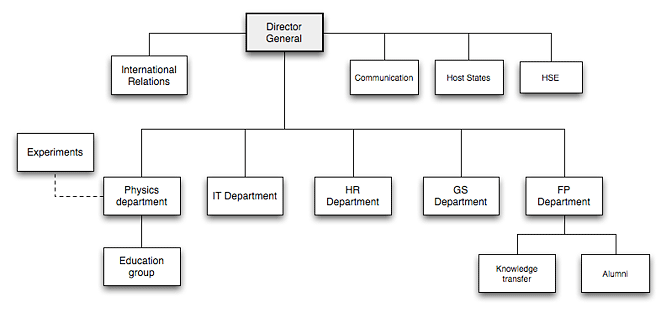
\includegraphics[scale=0.5]{cern_organogram}
				\end{center}
				\caption[Organigramma del CERN]{Organigramma ad alta granularità dell'organizzazione CERN.}
				\label{fig:cern_organogram}
			\end{figure}
			
			\paragraph{Indico}Il progetto Indico, oggetto di questa tesi, è così collocato all'interno della struttura del \ac{CERN}: \ac{IT} - \acs{CIS} - \acs{AVC} - Indico. Indico fa quindi, innanzitutto, parte del dipartimento \ac{IT}, ovvero il dipartimento dei servizi informatici al \ac{CERN} (il cui Department Head è Frédéric Hemmer). Quindi, Indico fa parte del gruppo \acr{CIS} che si occupa dei servizi di collaborazione come videoconferenze, pubblicazioni elettroniche, e servizi di gestione dei documenti. Il Group Leader del gruppo \ac{CIS} è Tim Smith. Più nel dettaglio, Indico fa parte della sezione \acr{AVC}, la quale si occupa di servizi per le videoconferenze e la gestione di eventi, sotto la supervisione del Section Leader Thomas Baron. Come vedremo più in dettaglio nel Capitolo \ref{chap:indico}, Indico è proprio il progetto che si occupa della gestione dell'applicazione web (o web application) per la creazione e gestione di eventi (come conferenze, meeting, ecc\dots). Durante la permanenza del sottoscritto al \ac{CERN}, il Project Manager di Indico è stato prima Jose Benito Gonzales e quindi Pedro Ferreira, il quale è stato anche supervisore del sottoscritto per tutta la durata del progetto.
		
		\subsection{Knowledge Transfer} \label{subsec:C;l;KT}
		
			Il gruppo \ac{KT}, parte del dipartimento \ac{FP}, si occupa si organizzare, catturare e distribuire la conoscenza e la tecnologia all'interno e fuori dal \ac{CERN}. Uno degli obiettivi è quello, ad esempio, di applicare i risultati scientifici ottenuti al \ac{CERN} in altri campi, come ad esempio la medicina (si stanno studiando, ad esempio, possibili tecnologie per la rimozione di tumori utilizzando piccoli acceleratori di particelle). Spesso, invece, quello che il gruppo \ac{KT} si prefigge di fare è rendere qualche prodotto o tecnologia \ac{CERN} più accessibile al mondo esterno, come università o aziende.
			
			Proprio questo era il fine dei fondi che il gruppo \ac{KT} ha destinato al progetto Indico. L'obiettivo era quello di rendere Indico più accessibile alle istituzioni e alle aziende che lo volessero utilizzare al di fuori del \ac{CERN} e di renderlo più facile da utilizzare. Ma di questo parleremo ampiamente nella Parte \ref{part:indico_KT_project} di questa tesi.

		\chapter{Indico} \label{chap:indico}
	
	Indico è una web application che fornisce strumenti per l'organizzazione di eventi di qualsiasi dimensione, da semplici lezioni a grandi conferenze. Prese vita nel 2002 come progetto europeo, per poi venir adottato dal \ac{CERN} nel 2004 come software per la gestione di eventi. Dal 2004 ad oggi, il \ac{CERN} è stato il principale finanziatore del progetto Indico, dedicando un team al suo sviluppo e supporto.
	
	\begin{figure}[h!]
		\begin{center}
			
\includegraphics[scale=1]{indico_logo.png}
		\end{center}
		\caption[Logo di Indico]{Logo di Indico.}
		\label{fig:indico_logo}
	\end{figure}
	
	Indico è uno strumento open source\footnote{Il codice aggiornato di Indico, e di tutti i progetti ad esso correlati, può essere trovato all'indirizzo \url{https://github.com/indico}.}, il che vuol dire non soltanto che è completamente gratuito, ma anche che altre istituzioni o individui al di fuori del \ac{CERN} possono ispezionarne il codice, contribuire allo sviluppo o modificarlo secondo le proprie preferenze.
	
	Indico viene quindi utilizzato da centinaia di istituzioni e organizzazioni in tutto il mondo, ma il principale utilizzatore rimane il \ac{CERN} stesso, che lo utilizza ogni giorno per gestire più di 300.000 eventi di diversa complessità e circa 200 stanze per conferenze e riunioni. L'istanza di Indico installata al \ac{CERN} prende il nome di Indico@CERN, raggiungibile all'indirizzo \url{http://indico.cern.ch/}. Inoltre, al \ac{CERN} è installata anche una seconda istanza minore di Indico utilizzata per prenotare gli uffici Burotel.
	
	\section{Principali caratteristiche} \label{sec:i;caratteristiche}
	
		Con Indico si possono gestire eventi di qualsiasi complessità: lezioni, riunioni, seminari e conferenze. Indico fornisce all'utente, durante tutta la fase di creazione e modifica di un evento, tutta una serie di strumenti per agevolare queste operazioni: l'utente può decidere secondo quali criteri far registrare terzi al suo evento, oppure come gestire l'invio di pubblicazioni o di materiale relativo all'evento.
		
		\paragraph{UI}Indico utilizza anche una potente e immediata interfaccia utente che si basa sul design \acr{WYSIWYG}. Grazie a questa \acr{UI} sarà facilissimo eseguire azioni altrimenti più complesse e tediose: la definizione di un form di registrazione per l'evento, la gestione delle timetables (Figura \ref{fig:indico_timetable}), che implementano un'intuitiva interfaccia drag-and-drop, oppure editor di testo che permettono l'utilizzo di rich text o formule matematiche.

		\begin{figure}[h!]
			\begin{center}
				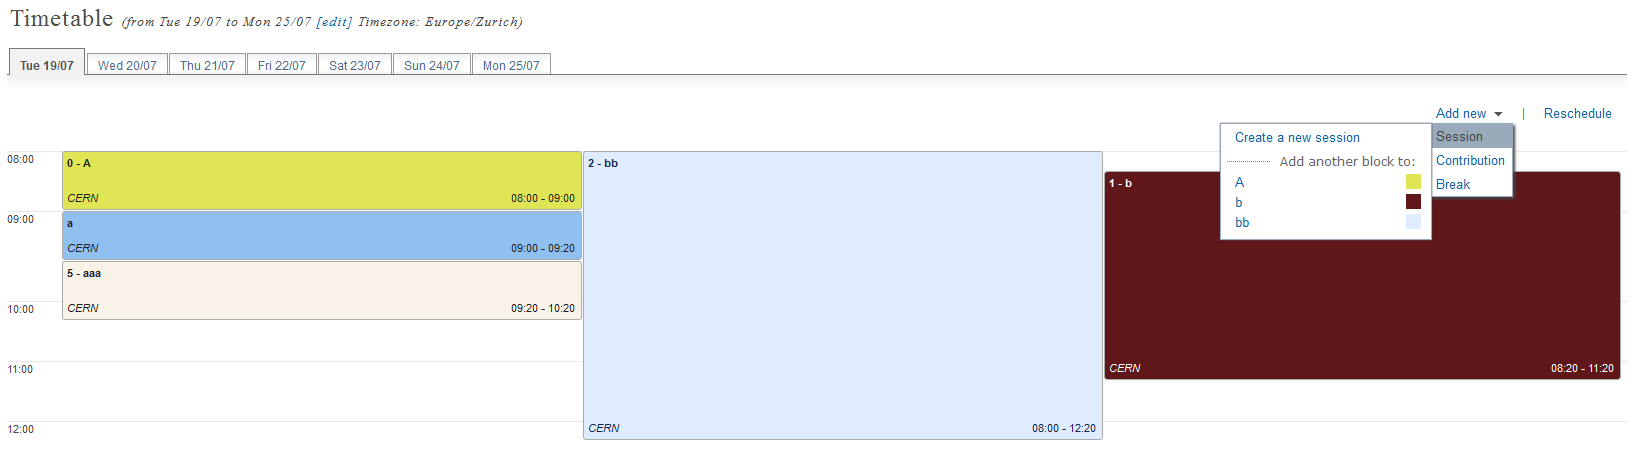
\includegraphics[scale=0.3]{indico_timetable.png}
			\end{center}
			\caption[Timetable in Indico (esempio)]{Un esempio di timetable di una conferenza in Indico.}
			\label{fig:indico_timetable}
		\end{figure}
		
		\paragraph{Struttura}Indico, ed il suo sistema di protezione, è organizzato in una struttura ad albero per categorie. Indico è stato sviluppato principalmente per grandi aziende, per questo gli eventi, ed il materiale ad essi associato, sono organizzati secondo una struttura gerarchica di categorie. L'amministratore del sistema potrà decidere ed assegnare livelli di protezione alle varie categorie secondo diversi livelli di granularità.

		\begin{figure}[h!]
			\begin{center}
				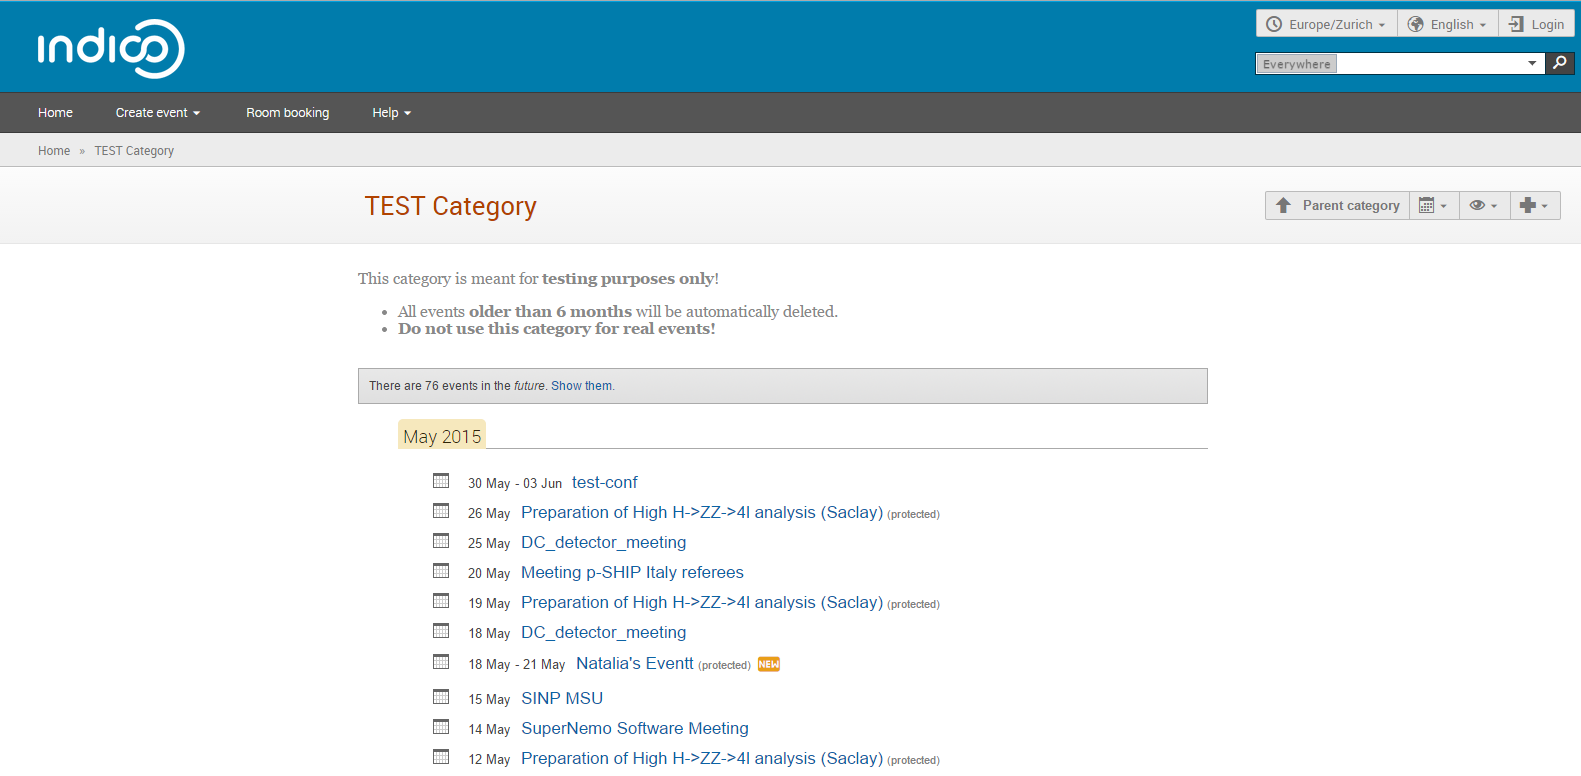
\includegraphics[scale=0.3]{indico_category.png}
			\end{center}
			\caption[Categoria in Indico (esempio)]{Un esempio di categoria con una serie di eventi al suo interno.}
			\label{fig:indico_category}
		\end{figure}
		
		\paragraph{Ricerca}In Indico è incluso anche un potente sistema di ricerca, che permette di ricercare gli eventi desiderati tramite poche parole chiave o osservare gli eventi previsti per un determinato periodo di tempo. Inoltre, tramite la dashboard, è possibile accedere velocemente a tutti gli eventi a cui l'utente è iscritto o che sta osservando.
		
		\paragraph{Room booking}Le compagnie e le organizzazioni, specialmente le più grandi, hanno spesso bisogno di gestire, limitare e tener traccia dell'utilizzo delle varie stanze e siti al loro interno. Per questo Indico include un potente ed intuitivo modulo per la prenotazione delle stanza (in inglese, room booking) che permette all'utente di specificare le caratteristiche di una stanza, approvare o meno la prenotazione di certe stanze e gestire strumenti e materiale messi a disposizione di certe stanza, come dispositivi audiovisivi per le video conferenze.
		
		\paragraph{Chat \& Video}Per rendere la gestione online di riunioni e conferenze ancora più efficiente, Indico integra perfettamente Vidyo\footnote{\url{http://it.vidyo.com/}.}, uno strumento per le videoconferenze, e permette di associare delle chatrooms Jabber/XMPP agli eventi.

		\begin{figure}[h!]
			\begin{center}
				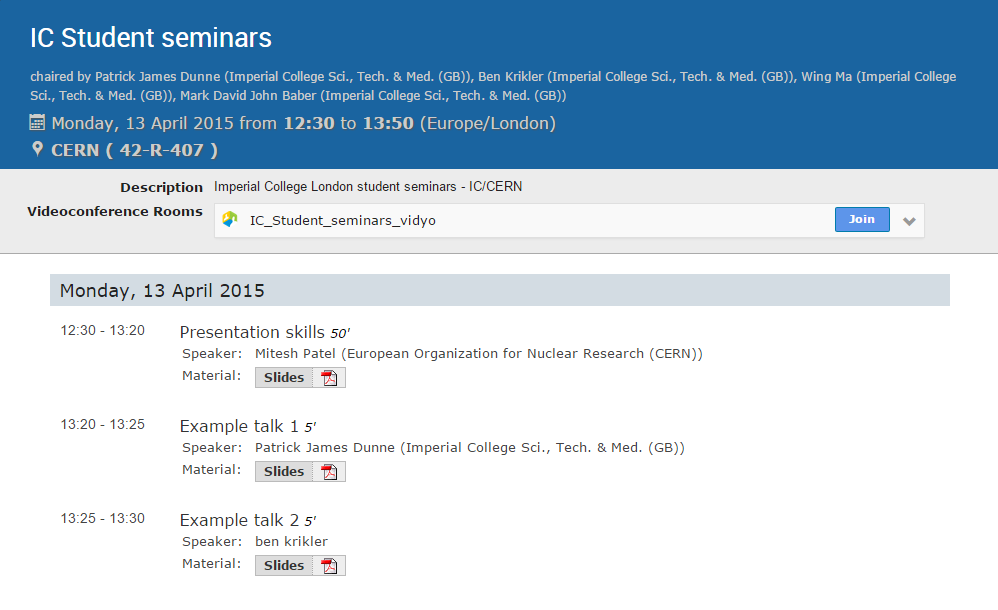
\includegraphics[scale=0.5]{indico_meeting.png}
			\end{center}
			\caption[Meeting in Indico (esempio)]{Un esempio di riunione in Indico con una videoconference room Vidyo associata.}
			\label{fig:indico_meeting}
		\end{figure}
		
		\paragraph{API}Dal momento che Indico è stato creato per agevolare la collaborazione e lo scambio di dati, tutte le informazioni contenute in Indico non sono esclusive di Indico stesso, ma possono essere recuperate (una volta accertato di avere l'accesso a quelle informazioni) tramite una semplice \acr{API}. Quest'\ac{API} è garantita essere RESTful  (dove \acs{REST} significa \aclu{REST}) ed è in costante aggiornamento.
		
	\section{Dettagli tecnici} \label{sec:i;dettagli_tecnici}
	
		Indico è un'applicazione web scritta principalmente in Python e Javascript (si veda la Figura \ref{fig:indico_languages}).
		
		\begin{figure}[h!]
			\begin{center}
				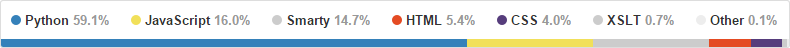
\includegraphics[scale=0.6]{indico_languages.png}
			\end{center}
			\caption[Linguaggi di Indico]{Una statistica dei linguaggi utilizzati nel codice di Indico (come mostrata su Github).}
			\label{fig:indico_languages}
		\end{figure}
		
		Essendo un'applicazione web, Indico implementa un web server ed un \ac{DB} per gestire le richieste dell'utente e recuperare i dati richiesti.
		
		\paragraph{WSGI}Indico utilizza \acr{WSGI} per gestire il web server. \ac{WSGI} è un'interfaccia standard tra web server e applicazioni Python, ovvero un'astrazione per rendere la comunicazione tra le due parti più semplice e modulare. In questo modo il server e  l'applicazione sono completamente separati e seguono lo standard. Ad esempio per Indico@CERN si utilizza Apache come web server, ma un amministratore di un'altra istanza può scegliere un altro server se lo desidera, in quanto \ac{WSGI} si configura senza problemi con quasi tutti gli web server in circolazione. \cite{indico:wsgi}
		
		\paragraph{DB}Prima dell'inizio del periodo di Techical Student, Indico utilizzava \acr{ZODB} come database. \ac{ZODB} è un database object-oriented che immagazzina oggetti Python. Dai primi del 2014 è invece stata iniziata una fase di migrazione, in  quanto \ac{ZODB} presentava alcuni svantaggi, come la difficoltà di eseguire query, la non indicizzazione dei record e il fatto di poter essere utilizzabile soltanto con Python. Dopo alcuni mesi di ricerca su quale potesse essere il miglior candidato per sostituire \ac{ZODB}, si è scelto PostgreSQL (spesso detto Postgres) come vincitore. Postgres è un \acr{ORDBMS}, ovvero un database relazionale a oggetti, che garantirà prestazioni più elevate durante l'utilizzo di Indico. Ovviamente passare da un database ad un altro non è una cosa semplice, in quanto tutto il codice dove si comunica con il \ac{DB} dev'essere adeguato al nuovo database. Migrare l'intero \ac{DB} di Indico@CERN in sol colpo era quindi un'impresa del tutto on fattibile. Si è optato quindi per una migrazione modulare: il processo di migrazione durerà circa un anno, durante il quale Indico utilizzerà un sistema di gestione del \ac{DB} ibrido \ac{ZODB}+Postgres, migrando modulo per modulo. \cite{indico:zodb}\cite{pedro:chep}
		
		\paragraph{Flask}Flask è un micro framework per applicazioni web, scritto in Python e basato su Werkzeug e Jinja2. Uno dei principali vantaggi offerti da Flask è l'URL Routing, ovvero la  possibilità di gestire gli URL in modo dinamico. Si possono associare diversi template per ogni tipo di richiesta ricevuta dal server, in modo da generare una pagina dinamica a seconda degli argomenti passati da Flask al template engine. \cite{indico:flask}
		
		\paragraph{Template engine(s)}Un template engine è uno strumento che permette di creare documenti personalizzati e dinamici a partire da un template (ovvero un modello) di base e dei dati di input. In questo caso, quando si parla di template engines, ci si riferisce a strumenti che generano pagine web secondo un certo modello inserendovi dei dati dinamici. Indico ha utilizzato per molti anni Mako come template engine ma in questi ultimi anni sta lentamente passando a Jinja2. \cite{indico:template_engines}
		
		\paragraph{Altre}A parte queste tecnologie citate, Indico ha iniziato a impiegare, nel corso degli ultimi anni, altri strumenti degni di nota, come  ad esempio WTForms, per la gestione dei campi dei form (ad esempio form di registrazione), SQLAchemy, ovvero un toolkit open source SQL, ed Alembic, uno strumento per la migrazione di database da utilizzare con SQLAlchemy.
		
	\section{La community} \label{sec:i;community}
	
		Come già accennato,  Indico è un software open source. Il suo codice sorgente più aggiornato è infatti disponibile su Github, all'indirizzo \url{https://github.com/indico/indico}. Il fatto di essere open source ha portato centinaia di organizzazioni e istituzioni, soprattutto nel campo della fisica delle particelle come ad esempio \acr{INFN} e \acr{IHEP}, ad utilizzare Indico per la gestione dei propri eventi. Negli anni questo ha portato alla formazione di una vera e propria community di utilizzatori (user e admin) di Indico.
		
		Questa commuity non soltanto utilizza Indico per i propri eventi, ma contribuisce anche allo sviluppo stesso del software,  inviando segnalazioni agli sviluppatori del team Indico  al \ac{CERN} sotto forma di ticket. Un ticket indica un problema da risolvere, o qualcosa da migliorare; risolvere il problema in questione o apportare la miglioria richiesta viene indicato con il termine di ``chiusura del ticket''.
		
		Altre volte invece, se chi si imbatte in un errore è uno sviluppatore a sua volta, può capitare che provi a risolvere il problema da solo, lavorando sul codice di Indico. Una volta  risolto, chi ha risolto il problema può inviare una cosiddetta \textit{pull request} tramite Github (il repository ufficiale che ospita il codice di Indico) agli sviluppatori di Indico al \ac{CERN}, in modo da indicare che  quel  problema è già stato risolto e possono includere (operazione di \textit{merge}) le modifiche apportate al codice principale di Indico.
	
	
	\part{Indico KT Project} \label{part:indico_KT_project}
		\chapter{KT Project: una panoramica} \label{chap:panoramica}

	In questo capitolo introdurremo i principali obiettivi del Progetto KT per Indico in modo da dare una panoramica generale dei sotto-progetti di cui il progetto principale è composto. Inoltre verranno esposti i principali strumenti e linguaggi utilizzati durante lo sviluppo del progetto.
	
	\section{Progetti principali} \label{sec:p;progetti_principali}
    	
    	Il progetto finanziato dal gruppo \ac{KT} per Indico, oggetto principale del programma di Technical Student a cui ha partecipato il sottoscritto, è nato come co-progetto tra i gruppi \ac{IT} e \ac{KT}. L'obiettivo principale di questo progetto era quello di migliorare la visibilità e l'impatto di Indico in tutto il mondo, in particolare al di fuori della comunità \acr{HEP}, all'interno della quale Indico si è già ampiamente affermato.
    	
    	Come si è già accennato nel Capitolo \ref{chap:CERN}, il concetto di \ac{KT} si basa sull'idea della diffusione e condivisione della conoscenza e degli strumenti necessari per ottenerla. L'idea alla base del progetto era quindi quella di modificare e migliorare il software Indico in modo da permettere una miglior diffusione dello stesso nel mondo. Per fare questo, il KT Project si era prefissato tre obiettivi generali da raggiungere:
    	
    	\begin{itemize}
        	\item rendere Indico più accessibile agli utenti
        	\item rendere Indico più semplice da utilizzare e personalizzare
        	\item rendere Indico, in generale, più moderno e visivamente ``attraente''
    	\end{itemize}
    	
    	Gli obiettivi prefissati col Progetto KT erano quindi molto ampi e generali e, come ci può immaginare, anche piuttosto complessi da mettere in pratica. Per questa ragione il progetto che è stato assegnato al sottoscritto non era che il primo di una serie di progetti, finanziati dal gruppo \ac{KT}, al fine di migliorare l'impatto a livello mondiale del software Indico. Infatti, durante il periodo dei 14 mesi passati a Ginevra dal sottoscritto, erano stati approvati e finanziati già due progetti dal gruppo \ac{KT} per Indico: il primo, assegnato al sottoscritto, ed un secondo da assegnare ad un futuro membro del team Indico, molto probabilmente un altro Techical Student.
    	
    	Il primo Progetto KT per Indico è stato quindi pianificato e suddiviso in una serie di sotto-progetti, i quali dovevano essere terminati durante i 12 (poi diventati 14) mesi del programma Technical Student (si veda \cite{pedro:gist} per la prima stesura del progetto). Quattro di questi sotto-progetti sono risultati essere più importanti e complessi degli altri e sono andati ad occupare la maggior parte del periodo di Technical Student. Di seguito ne parleremo brevemente per avere un'idea generale dei progetti principali del KT Project, mentre nei Capitoli successivi vedremo in dettaglio ognuno di essi.
    	
    	\subsection{Cloud Deployment} \label{subsec:p;pp;cloud}
    	
        	La prima fase del Progetto KT riguardava il Cloud Deployment di Indico, ovvero l'automatizzazione del processo di installazione e configurazione di Indico sia in ambiente cloud che in ambiente virtuale.
        	
        	Il progetto è durato circe un mese e mezzo, dal 23 Ottobre al 9 Dicembre 2013, ed ha portato alla stesura di due script fabric, uno per la creazione di immagini virtuali ed uno di gestione remota, ed una recipe cloud-init, per il deployment su struttura cloud.
    	
    	\subsection{Distribuzione e Packaging} \label{subsec:p;pp:distribuzione}
    	
        	Il secondo progetto del KT Project riguardava invece Distribuzione e Packaging, ovvero l'automatizzazione della creazione di diverse distribuzioni di Indico, sia dei sorgenti che precompilate, basate su diverse versioni sia di Indico che di Python e, successivamente, il caricamento di queste distribuzioni su un server e su GitHub.
        	
        	Questo progetto è durato circa due settimane, dal 27 Gennaio all'11 Febbraio 2014 ed il risultato è stato lo sviluppo di uno script fabric che automatizza l'intero processo di distribuzione.
    	
    	\subsection{Instance Tracking} \label{subsec:p;pp;instance_tracker}
    	
        	Il progetto sull'Instance Tracking si occupava invece di sviluppare un'applicazione web stand-alone per il tracciamento delle istanze di Indico e la successiva analisi statistica delle informazioni raccolte.
        	
        	Questo progetto, tra tutti, si è dimostrato essere il più importante, richiedendo 4 mesi di sviluppo, dall'11 Febbraio al 10 Giugno 2014. Il risultato di questo progetto è stato lo sviluppo di un'applicazione di tracciamento, successivamente denominata ``Cephalopod''.
    	
    	\subsection{Conference Customization Prototype} \label{subsec:p;pp;conference_customization_prototype}
    	
        	L'ultimo progetto era incentrato invece sullo sviluppo di un prototipo che aiutasse il team di Indico a decidere come sviluppare, in futuro, una nuova versione del tool per la personalizzazione delle conferenze.
        	
        	Sebbene non molto incisivo dal punto di vista dello sviluppo, quest'ultimo progetto è risultato molto impegnativo in quanto è stato caratterizzato da continui cambi di programma e frequenti sessioni di brainstorming con l'intero team di sviluppo. Quest'ultima fase è durata in totale circa 5 e mezzo, dal 10 Giugno a fine Novembre 2014.
    	
    \section{Strumenti e linguaggi} \label{sec:p;strumenti_linguaggi}
    
        Con questa ultima Sezione introduttiva, intendiamo fornire al lettore una serie di conoscenze e nozioni di base utili a capire il lavoro svolto con questo progetto. Indico infatti è composto da molti linguaggi diversi ed utilizza molti strumenti, sviluppati da terzi, senza i quali non potrebbe funzionare. È necessario quindi sapere quali sono e cosa fanno ognuno di questi strumenti, nonché essere a conoscenza dei linguaggi utilizzati.
        
        \subsection{GitHub} \label{subsec:p;sl;github}
        
            GitHub è un servizio web per l'hosting di repository Git\footnote{Git è un noto sistema per la gestione del codice e lo sviluppo di applicazioni sviluppato da Linus Torvalds.}. Github offre le funzionalità caratteristiche di Git, come controllo di versione distribuito o gestione del codice sorgente. Tuttavia, a differenza di Git che è soltanto uno strumento da linea di comando, Github offre un'interfaccia grafica basata sul web. Inoltre fornisce molte funzionalità incentrate sulla collaborazione di più sviluppatori, come tracciamento dei bug, richiesta di funzionalità, gestione delle attività e pagine wiki per ogni progetto.
            
        	\begin{figure}[h!]
        		\begin{center}
        			
\includegraphics[scale=0.2]{octocat.png}
        		\end{center}
        		\caption[Octocat]{Octocat, la mascotte ufficiale di GitHub.}
        		\label{fig:octocat}
        	\end{figure}
        	
        	GitHub offre opzioni sia per repository privati, a pagamento, che pubblici, completamente gratuiti. Quest'ultimi vengono solitamente utilizzati per ospitare progetti software open source, come nel caso di Indico.
        	
        	In GitHub si possono creare profili utente, al quale si accede tramite delle credenziali, o organizzazioni, che rappresentano la collaborazione di più individui. Ogni utente e ogni organizzazione può definire una serie di repository, pubblici o privati, condivisi o meno. La pagina GitHub dell'organizzazione Indico è ad esempio \url{https://github.com/indico}, mentre quella del sottoscritto \url{https://github.com/oddlord}. La pagina GitHub di Indico ospita molti progetti, tutti legati a Indico, ma che non sono necessariamente il progetto Indico principale: ad esempio il repository del progetto principale Indico si trova all'indirizzo \url{https://github.com/indico/indico}, mentre il progetto sul Cloud Deployment sviluppato dal sottoscritto è all'indirizzo \url{https://github.com/indico/indico-cloud-images}.
    
        \subsection{Python} \label{subsec:p;sl;python}
        
            Python è un linguaggio di programmazione dinamico, di alto livello, general-purpose e interpretato che, al momento, è molto diffuso e utilizzato, specialmente nel settore delle applicazioni web. La filosofia di Python tende a enfatizzare la leggibilità del codice, proponendo una sintassi tramite la quale il programmatore può scrivere programmi anche in poche linee di codice, cosa che sarebbe impossibile con linguaggi come C++ o Java. \cite{wiki:python}
        
        	\begin{figure}[h!]
        		\begin{center}
        			
\includegraphics[scale=0.6]{python_logo.png}
        		\end{center}
        		\caption[Logo di Python]{Logo di Python.}
        		\label{fig:python_logo}
        	\end{figure}
        	
        	Python supporta molti paradigmi di programmazione, tra i quali programmazione a oggetti, imperativa e funzionale/procedurale. Il sistema di tipaggio di Python è dinamico, ovvero la correttezza dei tipi dei vari oggetti viene stabilita in tempo di esecuzione.
        	
        	Indico è un software principalmente scritto in Python. Per questo motivo all'interno di questa tesi faremo riferimento spesso l'utilizzo di comandi o librerie Python, per descrivere lo sviluppo dei vari progetti che hanno composto il KT Project.
        
            Un importante comando offerto da Python è \python{.format()}, che sarà accennato all'interno del Capitolo \ref{chap:cloud_deployment}. Questa funzione sostituisce a degli speciali \textit{placeholder} (o segnaposti, in italiano), presenti nell'oggetto stringa sul quale viene eseguito, i valori associati ad ogni placeholder tramite un particolare dizionario, passato come unico argomento. I placeholder sono parole chiave che identificano un parametro in modo univoco racchiuse tra parentesi graffe. Il comando \python{.format()} funziona quindi come segue:
            
            \begin{center}
                \begin{lstlisting}[language=python, gobble=18]
                    data = {'first': 'Hodor', 'last': 'Hodor!'}
                    template = '{first} {last}'
                    result = template.format(**data)
                \end{lstlisting}
                \captionsetup{textformat=empty,labelformat=empty} \vspace{-2em}
                \captionof{lstlisting}[Comando \python{.format()} (esempio)]{Esempio del funzionamento del comando \python{.format()}.}
            \end{center}
            
            Il risultato salvato in \python{result} sarà quindi la stringa \python{'Hodor Hodor!'}.
        
        \subsection{Cloud-init} \label{subsec:p;sl;cloud-init}
        
            Cloud-init\footnote{\url{https://launchpad.net/cloud-init}.} è uno degli strumenti più utilizzati per l'inizializzazione e configurazione di server cloud. Tramite la compilazione di alcune semplici impostazioni, l'utente sarà in grado di avviare un nuovo server cloud specificando una serie di azioni da eseguire in automatico durante il primo avvio, come ad esempio eseguire determinati script, copiare alcuni file da remoto, installare pacchetti ed applicazioni necessarie, e così via. Cloud-init è installato di default su molte distribuzioni Linux, come Ubuntu, Fedora, Debian, CentOS, ecc. \cite{cloud-init:readthedocs}
            
            In poche parole, Cloud-init è un modulo che viene eseguito all'avvio di una macchina virtuale e permette di specificare delle azioni da eseguire tramite un file detto \textit{user-data}. Un file di questo tipo, ovvero che permette di specificare una serie di azioni che verranno eseguite in automatico, viene detto \textit{recipe} (ovvero ``ricetta'' in inglese). Si parla infatti di \textit{cloud-init recipe} riferendosi ad una particolare configurazione da passare a cloud-init.
            
            Per utilizzare una cloud-init recipe, è sufficiente specificare il file \bash{user-data} generato quando si avvia il server sul cloud per la prima volta. Il comando da usare varia a seconda del Cloud Service Provider scelto. Per infrastrutture cloud basate su tecnologia OpenStack, ad esempio, è sufficiente eseguire il seguente comando da terminale:
            
            \begin{center}
                \begin{lstlisting}[language=bash, gobble=18]
                    $ nova boot --image ubuntu-cloudimage --flavor 1 --user-data user-data
                \end{lstlisting}
                \captionsetup{textformat=empty,labelformat=empty} \vspace{-2em}
                \captionof{lstlisting}[Boot con cloud-init (esempio OpenStack)]{Esempio di comando di boot con cloud-init per infrastrutture basate su OpenStack.}
            \end{center}
            
            Tramite il file \bash{user-data} è possibile passare al modulo cloud-init una serie di file in diversi formati supportati, tra i quali:
            
            \begin{itemize}
                \item file compresso in formato \bash{.gzip};
                \item file \acr{MIME} multiparti;
                \item script bash;
                \item file cloud-config.
            \end{itemize}
            
            In particolare, i file gzip possono essere utili per ridurre le dimensioni del file \bash{user-data}, essendo questo limitato a 16KB. I file \ac{MIME} multiparti sono tipi di file composti che servono a raggruppare altri file, dei tipi sopra citati, in un unico file. I file di script servono ad eseguire una serie di comandi subito dopo il primo boot, mentre i file cloud-config sono particolari file utilizzati per copiare file in remoto sulla macchina sul cloud oppure per installare tutti i pacchetti aggiuntivi necessari.
            
            Come vedremo nel Capitolo \ref{chap:cloud_deployment}, le recipe cloud-init sono state molto utili per la fase di Cloud Deployment di Indico.
                    
        \subsection{Fabric} \label{subsec:p;sl;fabric}
        
            Fabric è una ``libreria Python e uno strumento da linea di comando per rendere più semplice l'uso di \acr{SSH} per applicazioni di deployment o operazioni di amministrazione di sistema''. \cite{fabric:documentation}
            
        	\begin{figure}[h!]
        		\begin{center}
        			
\includegraphics[scale=1]{fabric_logo.png}
        		\end{center}
        		\caption[Logo di Fabric]{Logo di Fabric.}
        		\label{fig:fabric_logo}
        	\end{figure}
            
            Fabric fornisce una serie di comandi per l'esecuzione sia locale che remota di comandi shell (normali o tramite \bash{sudo}), per l'upload o il download di file o per l'esecuzione di operazioni ausiliare, come richiedere un input all'utente o bloccare l'esecuzione di un'operazione in esecuzione.
            
            Uno script fabric è quindi un semplice script python, dove però si possono utilizzare tutti i comandi messi a disposizione da Fabric. Due comandi fabric molto importanti sono \python{local(cmd)} e \python{run(cmd)}. Entrambi i comandi eseguono il comando \python{cmd} passato come argomento come comando shell, l'unica differenza tra i due è che \python{local(cmd)} esegue \python{cmd} in locale, ovvero sulla macchina che sta eseguendo lo script fabric, mentre \python{run(cmd)} esegue \python{cmd} su una macchina remota, opportunamente specificata. Inoltre un altro comando molto utile è il comando \python{put(file, dest)} che permette di copiare il file \python{file}, che si trova sulla macchina locale, nella destinazione \python{dest} all'interno della macchina remota, quindi mimando il comportamento del comando \bash{scp} di bash.
            
            Per permettere una stesura più semplice e meno ridondante di uno script fabric, è possibile specificare alcune opzioni in un particolare dizionario, detto \textit{ambiente} e denotato dalla variabile \python{env}, in modo da non doverle ripetere ogni volta che si invoca un comando fabric. Ad esempio specificando un valore per il campo \python{env.hosts} possiamo definire una volta per tutte l'indirizzo di tutte le macchine remote su cui vogliamo eseguire i comandi passati a \python{run()}, senza dover stare a ripeterli inutilmente ogni volta.
            
            Ogni script fabric deve specificare delle operazioni, dette \textit{task}, che possono poi essere eseguite da linea di comando. Ogni task è una funzione python contrassegnata dal decoratore \python{@task}, che contraddistingue le task (operazioni che possono essere eseguite dall'utente) da funzioni interne dello script.
            
            Per poter essere eseguito, uno script fabric deve essere chiamato \bash{fabfile.py}. Per eseguire quindi uno script fabric basta eseguire un comando della forma seguente:
            
            \begin{center}
                \begin{lstlisting}[language=bash, gobble=18]
                    $ fab task1 task2
                \end{lstlisting}
                \captionsetup{textformat=empty,labelformat=empty} \vspace{-2em}
                \captionof{lstlisting}[Esecuzione task fabric (esempio)]{Esempio dell'esecuzione di due task fabric.}
            \end{center}
            
            Un comando come quello appena mostrato esegue prima la task \bash{task1} e quindi \bash{task2} definite nel file \bash{fabfile.py}.
            
            Fabric verrà utilizzato, all'interno del progetto di Cloud Deployment, per la stesura sia di uno script per la creazione automatica di immagini virtuali che di uno script per la gestione remota di macchine cloud. Inoltre sarà utilizzato anche per la fase di Distribuzione e Packaging.
        
        \subsection{QEMU e KVM} \label{subsec:p;sl;qemu_kvm}
        
            \acr{QEMU} è un emulatore e strumento di virtualizzazione open source. \acr{KVM} invece è anch'esso uno strumento di virtualizzazione e fornisce anche delle funzionalità di accelerazione hardware per sistemi Linux.
            
            \ac{QEMU} e \ac{KVM} possono essere utilizzati in congiunzione, tant'è che \ac{KVM} viene distribuito da anni assieme a \ac{QEMU}. Si potrebbe pensare di utilizzare soltanto uno di questi due strumenti per lavorare con macchine virtuali, tuttavia, anche se \ac{QEMU} fornisce un sistema di virtualizzazione completo e a se stante, per applicazioni pratiche è spesso necessario affiancargli \ac{KVM} per migliorarne le performance. D'altro canto, \ac{KVM} soltanto non fornisce tutte le funzionalità di un ambiente di virtualizzazione completo come \ac{QEMU}.
            
            \ac{QEMU} e \ac{KVM} sono stati utilizzati durante la fase di Cloud Deployment del progetto, ed in particolare nello script di creazione di immagini virtuali, come vedremo all'interno del Capitolo \ref{chap:cloud_deployment}.
            
            Per maggiori informazioni su \ac{QEMU} e \ac{KVM} si consultino \cite{kvm:wiki} e \cite{qemu:wiki}.
        
        \subsection{Requests} \label{subsec:p;sl;requests}
        
            Requests è una delle più semplici, in termini di utilizzo, librerie \acr{HTTP} per Python.
            
            Grazie a Requests si possono fare richieste, o inviare dati, tramite il protocollo \ac{HTTP} scrivendo solo poche linee di codice, in piena filosofia Python. Se ad esempio volessimo ottenere la lista degli eventi pubblici di GitHub, basterebbe scrivere la seguente linea di codice:
            
            \begin{center}
                \begin{lstlisting}[language=python, gobble=18]
                    r = requests.get('https://api.github.com/events')
                \end{lstlisting}
                \captionsetup{textformat=empty,labelformat=empty} \vspace{-2em}
                \captionof{lstlisting}[\python{get()} con Requests (esempio)]{Esempio del comando \python{get()} della libreria Requests.}
            \end{center}
            
            All'interno della variabile \python{r} sarà quindi presente la risposta ottenuta dall'esecuzione di quella richiesta. La risposta ad una richiesta può essere di svariati tipi e solitamente contiene tutti i dati richiesti, opportunamente strutturati. Nell'esempio di sopra la risposta sarà in formato \acr{JSON}.
            
            L'esempio opposto riguarda invece l'invio di dati tramite un'\ac{API}. Per inviare dei dati basta semplicemente utilizzare il comando \python{post()}, come mostrato dall'esempio seguente:
            
            \begin{center}
                \begin{lstlisting}[language=python, gobble=18]
                    r = requests.post('http://httpbin.org/post', data = {'key':'value'})
                \end{lstlisting}
                \captionsetup{textformat=empty,labelformat=empty} \vspace{-2em}
                \captionof{lstlisting}[\python{post()} con Requests (esempio)]{Esempio del comando \python{post()} della libreria Requests.}
            \end{center}
            
            Requests verrà utilizzata ampiamente all'interno del progetto di Instance Tracking (Capitolo \ref{chap:instance_tracker}) e anche durante la fase di upload a GitHub del progetto di Distribuzione e Packaging (Capitolo \ref{chap:distribuzione_packaging}).
        
        \subsection{Twitter Bootstrap} \label{subsec:p;sl;twitter_bootstrap}
        
            Bootstrap\footnote{\url{http://getbootstrap.com/}.}, sviluppato da Twitter, è uno dei più famosi framework \ac{HTTP}, \acr{CSS} e Javascript per sviluppare progetti web dinamici e reattivi e dal design moderno.
            
            Scaricando i file di Bootstrap ed includendoli nel progetto, uno sviluppatore web ha accesso a tutta una serie di stili, elementi \acr{HTML} e funzioni Javascript che gli permettono, in poche linee di codice, di creare da zero un sito dinamico e moderno.
            
            Bootstrap, ad esempio, include un set di icone, dette Glyphicons, dallo stile minimalista e gradevole. Tramite il codice seguente, ad esempio, si produce il bottone in Figura \ref{fig:button_bootstrap}.
            
            \begin{center}
                \begin{lstlisting}[language=html, gobble=18]
                    <button type="button" class="btn btn-default btn-lg">
                        <span class="glyphicon glyphicon-star" aria-hidden="true"></span> Star
                    </button>
                \end{lstlisting}
                \captionsetup{textformat=empty,labelformat=empty} \vspace{-2em}
                \captionof{lstlisting}[Bottone con Bootstrap (esempio)]{Esempio della definizione di un bottone con icona con Bootstrap.}
            \end{center}
            
        	\begin{figure}[h!]
        		\begin{center}
        			
\includegraphics[scale=1]{button_bootstrap.png}
        		\end{center}
        		\caption[Bottone con Bootstrap (esempio)]{Esempio di un bottone con icona con Bootstrap.}
        		\label{fig:button_bootstrap}
        	\end{figure}
        	
        	Un bottone così definito risulta avere uno stile dinamico, ad esempio diventa ombreggiato al passaggio del mouse e rientra quando viene cliccato.
        	
        	Un altro esempio possono essere i menu a tendina. Tramite il frammento di codice \ac{HTML} seguente, ad esempio, si genera un menu a tendina come in Figura \ref{fig:dropdown_bootstrap}.
        	
        	
            \begin{center}
                \begin{lstlisting}[language=html, gobble=18]
                    <div class="dropdown">
                        <button class="btn btn-default dropdown-toggle" type="button" id="dropdownMenu1" data-toggle="dropdown" aria-haspopup="true" aria-expanded="true">
                            Dropdown
                            <span class="caret"></span>
                        </button>
                        <ul class="dropdown-menu" aria-labelledby="dropdownMenu1">
                            <li><a href="#">Action</a></li>
                            <li><a href="#">Another action</a></li>
                            <li><a href="#">Something else here</a></li>
                            <li role="separator" class="divider"></li>
                            <li><a href="#">Separated link</a></li>
                        </ul>
                    </div>
                \end{lstlisting}
                \captionsetup{textformat=empty,labelformat=empty} \vspace{-2em}
                \captionof{lstlisting}[Menu a tendina con Bootstrap (esempio)]{Esempio della definizione di un menu a tendina con Bootstrap.}
            \end{center}
            
        	\begin{figure}[h!]
        		\begin{center}
        			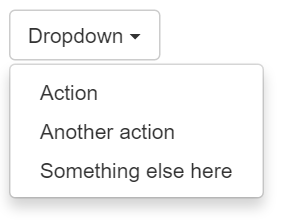
\includegraphics[scale=1]{dropdown_bootstrap.png}
        		\end{center}
        		\caption[Menu a tendina con Bootstrap (esempio)]{Esempio di un menu a tendina con Bootstrap.}
        		\label{fig:dropdown_bootstrap}
        	\end{figure}
        	
        	Bootstrap sarà utilizzato come stile di base per l'applicazione sviluppata durante il progetto di Instance Tracking, descritto all'interno del Capitolo \ref{chap:instance_tracker}.
        
        \subsection{Flask} \label{subsec:p;sl;flask}
        
            Flask\footnote{\url{http://flask.pocoo.org/}.} è un microframework per sviluppare applicazioni web in Python basato su Werkzeug e Jinja2.
            
            Un esempio minimale di applicazione è il frammento di codice seguente, che immaginiamo essere memorizzato all'interno del file \bash{hello.py}:
            
            \begin{center}
                \begin{lstlisting}[language=python, gobble=18]
                    from flask import Flask
                    app = Flask(__name__)
                    
                    @app.route("/")
                    def hello():
                        return "Hello World!"
                    
                    if __name__ == "__main__":
                        app.run()
                \end{lstlisting}
                \captionsetup{textformat=empty,labelformat=empty} \vspace{-2em}
                \captionof{lstlisting}[Applicazione in Flask (esempio)]{Esempio della definizione di un'applicazione con Flask.}
            \end{center}
            
            L'applicazione può quindi essere avviata eseguendo la seguente istruzione da linea di comando:
            
            \begin{center}
                \begin{lstlisting}[language=bash, gobble=18]
                    $ python hello.py
                     * Running on http://localhost:5000/
                \end{lstlisting}
                \captionsetup{textformat=empty,labelformat=empty} \vspace{-2em}
                \captionof{lstlisting}[Esecuzione dell'applicazione in Flask (esempio)]{Esempio di esecuzione dell'applicazione con Flask.}
            \end{center}
            
            Quindi, accedendo all'\ac{URL} \html{http://localhost:5000/}, si vedrà stampata sul browser la stringa \html{Hello World!}.
            
            Flask mette a disposizione dello sviluppatore delle funzioni molto importanti, ad esempio per fare \textit{\ac{URL} routing} o \textit{template rendering}. L'azione di associare un \ac{URL} ad una funzione è detto \ac{URL} routing (ovvero ``indirizzamento degli \ac{URL}'') ed è resa disponibile grazie al decoratore di Flask \python{route()}. Una volta associato l'\ac{URL} alla funzione desiderata, la funzione può eseguire i comandi specificati ogni volta che si accede a tale \ac{URL}. In particolare, se l'\ac{URL} corrisponde alla visualizzazione di una pagina, allora tale funzione dovrà occuparsi di generare la pagina richiesta e quindi restituirla, utilizzando la funzione Flask \python{render_template()}. Il comando \python{render_template()} prende in input un file di template, scritto in Jinja2, ed un dizionario di variabili e restituisce il file istanziato, ovvero il template a cui sono stati sostituiti i valori dei parametri ai placeholder presenti nel template, in modo molto simile a quanto visto per \python{format()}. Inoltre, Flask mette a disposizione altre funzioni utili, come ad esempio la funzione \python{redirect()}, che serve a reindirizzare l'applicazione su un altro \ac{URL}, oppure il decoratore \python{login_required}, che permette di eseguire i comandi di una certa funzione se e solo se si chi richiede l'\ac{URL} è un utente correttamente registrato e loggato, restituendo altrimenti un errore.
            
            Flask è stato utilizzato come framework per Cephalopod, l'applicazione descritta all'interno del Capitolo \ref{chap:instance_tracker}, e per il prototipo sviluppato per la fase di Conference Customization (Capitolo \ref{chap:conference_customization_prototype}).
            
        \subsection{Jinja2} \label{subsec:p;sl;jinja2}
        
            Jinja2 è un template engine molto diffuso per Python compatibile con Flask.
            
            Uno dei vantaggi di Jinja2 è la possibilità di definire blocchi condizionali e cicli all'interno del template. Prendiamo ad esempio il seguente frammento di template scritto in sintassi Jinja2:
            
            \begin{center}
                \begin{lstlisting}[language=html, gobble=18]
                    <ul>
                        
                            <li><a href="{{ user.url }}">{{ user.username }}</a></li>
                        
                    </ul>
                \end{lstlisting}
                \captionsetup{textformat=empty,labelformat=empty} \vspace{-2em}
                \captionof{lstlisting}[Template in Jinja2 (esempio)]{Esempio della definizione di un template con Jinja2.}
            \end{center}
            
            Consideriamo quindi il seguente dizionario Python:
            
            \begin{center}
                \begin{lstlisting}[language=python, gobble=18]
                    {
                        'users': [
                            {'username': 'Tommy', 'url': 'www.tommy.com'},
                            {'username': 'Doge', 'url': 'www.dogetheking.org'},
                            {'username': 'The Guy', 'url': 'www.theguy.co.uk'}
                        ]
                    }
                \end{lstlisting}
                \captionsetup{textformat=empty,labelformat=empty} \vspace{-2em}
                \captionof{lstlisting}[Dizionario di parametri per il template (esempio)]{Esempio di dizionario di parametri per istanziare il template.}
            \end{center}
            
            Quindi, se a questo punto invochiamo il comando \python{render_template()} di Flask sul template e la lista appena definiti, otteniamo il seguente frammento di codice \ac{HTML}, che rappresenta l'istanziazione del template secondo i parametri passati:
            
            \begin{center}
                \begin{lstlisting}[language=html, gobble=18]
                    <ul>
                        <li><a href="www.tommy.com">Tommy</a></li>
                        <li><a href="www.dogetheking.org">Doge</a></li>
                        <li><a href="www.theguy.co.uk">The Guy</a></li>
                    </ul>
                \end{lstlisting}
                \captionsetup{textformat=empty,labelformat=empty} \vspace{-2em}
                \captionof{lstlisting}[Template in Jinja2 (esempio)]{Esempio della definizione di un template con Jinja2.}
            \end{center}
            
            Jinja2, in congiunzione con Flask, è stato utilizzato per lo sviluppo di Cephalopod, come vedremo all'interno del Capitolo \ref{chap:instance_tracker}.
        
        \subsection{PostgreSQL e SQLAlchemy} \label{subsec:p;sl;postgreSQL_SQLAlchemy}
        
            PostgreSQL\footnote{\url{http://www.postgresql.org/}.} è un potente database \acr{ORDBMS}, ovvero relazionale orientato a oggetti, open source. In commercio da più di 15 anni, PostgreSQL è disponibile per tutti i maggiori sistemi operativi, tra i quali Linux, Unix e Windows. Indico, al momento, utilizza un sistema di database ibrido, utilizzando sia \ac{ZODB} che PostgreSQL, migrando piano piano tutto il database su quest'ultimo.
            
        	\begin{figure}[h!]
        		\begin{center}
        			
\includegraphics[scale=0.5]{postgresql_logo.png}
        		\end{center}
        		\caption[Logo di PostgreSQL]{Logo di PostgreSQL.}
        		\label{fig:postgresql_logo}
        	\end{figure}
        	
        	SQLAlchemy\footnote{\url{http://www.sqlalchemy.org/}.}, invece, è un toolkit \acr{SQL} per Python, ovvero uno strumento che permette ad applicazioni Python di comunicare con database \ac{SQL}. Per maggiori informazioni sul supporto di SQLAlchemy a PostgreSQL si veda \cite{sqlalchemy:postgresql}.
        	
        	L'accoppiata PostgreSQL-SQLAlchemy è stata utilizzata per sviluppare Cephalopod, il tracciatore d'istanze descritto all'interno del Capitolo \ref{chap:instance_tracker}.
        
        \subsection{jqPlot} \label{subsec:p;sl;jqplot}
        
            jqPlot\footnote{\url{http://www.jqplot.com/}.} è un plugin Javascript per la visualizzazione di grafici. jqPlot permette di definire grafici interattivi e dinamici ed offre allo sviluppatore la possibilità di personalizzare ogni grafico tramite una vasta scelta di stili disponibili. Tra gli stili più noti troviamo il grafico a barre, il grafico a linea e il grafico a torta. Ad ogni grafico possono essere inoltre associate una serie di opzioni, per definirne l'aspetto ed il comportamento. Ci sono opzioni, ad esempio, per attivare o meno l'animazione del grafico, o per visualizzare delle etichette sui vari punti del grafico, o ancora per definire nuovi punti del grafico semplicemente cliccando col mouse.
            
            Il codice d'esempio seguente mostra quanto sia facile definire, con jqPlot, un grafico come quello in Figura \ref{fig:jqplot}.
            
            \begin{center}
                \begin{lstlisting}[language=javascript, gobble=18]
                    $(document).ready(function(){
                        var plot1 = $.jqplot ('chart1', [[3,7,9,1,5,3,8,2,5]]);
                    });
                \end{lstlisting}
                \captionsetup{textformat=empty,labelformat=empty} \vspace{-2em}
                \captionof{lstlisting}[Grafico con jqPlot (esempio)]{Esempio della definizione di un grafico a linea semplice con jqPlot.}
            \end{center}
            
        	\begin{figure}[h!]
        		\begin{center}
        			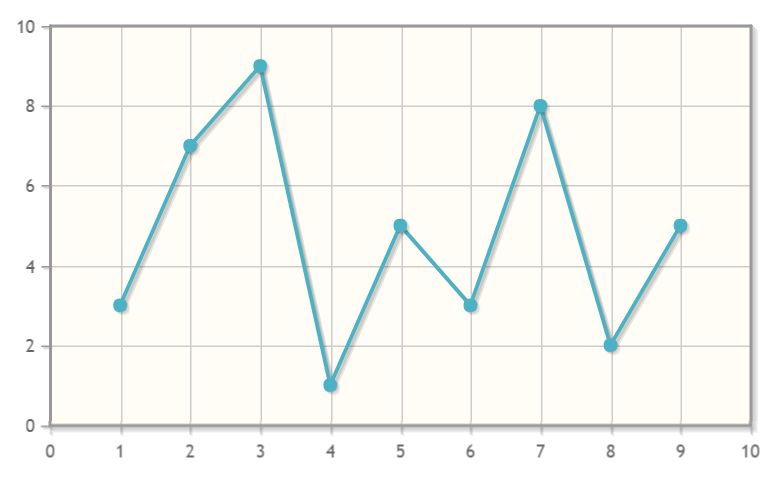
\includegraphics[scale=0.8]{jqplot.png}
        		\end{center}
        		\caption[Grafico con jqPlot (esempio)]{Esempio di un grafico a linea semplice con jqPlot (fonte \cite{jqplot:examples}).}
        		\label{fig:jqplot}
        	\end{figure}
        	
        	Per poter utilizzare le funzioni e gli stili offerti da jqPlot è sufficiente scaricare i sorgenti dal sito ufficiale di jqPlot, includerli all'interno della directory del progetto e quindi importare i file necessari all'interno del codice Javascript, che vogliamo produca il grafico, dell'applicazione che si sta sviluppando.
        	
        	jqPlot è stato utilizzato per sviluppare la pagina delle statistiche del tracciatore d'istanze (Capitolo \ref{chap:instance_tracker}) e per costruire la nuova pagina delle statistiche per Indico (Capitolo \ref{chap:altri_progetti}).

		\chapter{Cloud Deployment} \label{chap:cloud_deployment}

    I concetti di \textit{cloud} e \textit{virtualizzazione} stanno prendendo sempre più piede, nel corso degli ultimi anni, nel settore informatico ed in particolare nel campo di sviluppo software.
    
    L'idea alla base del cloud  si basa sul semplice fatto che molte volte un utente, o un amministratore di sistema, può voler essere in grado di eseguire una certa applicazione, senza però doversi preoccupare dell'hardware necessario. L'unica cosa che interessa è poter eseguire il software desiderato senza bisogno di doversi preoccupare dei dettagli tecnici quali installare un server, configurarlo, o anche pensare alle varie problematiche relative all'hardware come la capacità degli hard disk necessaria, di quanti processori ha bisogno, di quanta banda per la trasmissione dei dati, ecc. Per rispondere a questa esigenza, sono nati i \textit{Cloud Service Provider}, ovvero aziende in possesso di un grandissimo numero di macchine, molto capienti, molto potenti e molto veloci. In parole povere, quello che offrono i Cloud Service Provider, è di affittare le loro macchine per un certo costo mensile (o annuale, dipende dal tipo di contratto). Questi provider fanno scegliere all'utente il tipo di profilo desiderato: ci saranno ad esempio i bassi profili, che forniscono risorse limitate in cambio di un pagamento minimo, oppure alti profili, che forniscono all'utente un'altissima potenza di calcolo in cambio, ovviamente, di un pagamento più alto. L'utente si limita quindi a scegliere il profilo che più gli è consono e a ``lanciare'' (in inglese, \textit{deploy}) la propria applicazione sulla macchina appena affittata. Non sarà necessario quindi fare alcuna installazione fisica di macchine o hardware, né tanto meno mantenerle: il Cloud Service Provider scelto si occuperà di tutto questo, mentre l'utente potrà concentrarsi sulla gestione e sull'utilizzo della propria applicazione. Ovviamente, dato che facendo così l'utente si ``astrae'' dal concetto di macchina fisica, egli non saprà mai con certezza su che specifiche hardware viene effettivamente eseguita la sua applicazione. La sua applicazione potrebbe venire eseguita su un supercomputer molto potente, o magari su un una macchina più semplice dedicata solo a quell'applicazione. L'utente non lo sa ma, d'altro canto, nemmeno gli interessa, avendo scelto di lanciare la sua applicazione sul cloud. Addirittura spesso può anche capitare che, a seconda del carico di lavoro delle varie macchine del provider, l'applicazione venga prima eseguita su delle macchine e in un secondo momento su delle altre. Da questo il cloud prende il suo nome: un'applicazione lanciata sul cloud non risiede necessariamente in una macchina specifica, ma la possiamo immaginare all'interno di una sorta di ``nuvola'', ovvero in uno spazio indefinito all'interno del quale però l'applicazione ha accesso a tutte le risorse hardware richieste.
    
    L'idea della virtualizzazione è molto simile a quella del cloud ma orientata più al sistema operativo di una macchina. Sappiamo che spesso un'applicazione è ottimizzata per un certo sistema operativo o, addirittura, funziona soltanto se eseguita su determinati sistemi operativi. Per gli sviluppatori, spesso, è una scelta obbligata quella di prediligere alcuni sistemi operativi rispetto ad altri: infatti alcuni sistemi operativi possono essere talmente diversi tra loro che garantire la compatibilità dell'applicazione su tutti i sistemi operativi comporterebbe dover riprogettare e riscrivere l'applicazione da capo, il che non è sempre possibile, a seconda delle risorse disponibili per lo sviluppo. Per ovviare a questi problemi sono stati sviluppati degli appositi tools di virtualizzazione, come il ben noto Virtualbox di Oracle\footnote{\url{https://www.virtualbox.org/}}. I tool di virtualizzazione permettono di simulare un sistema operativo eseguendolo su una macchina fisica sulla quale è installato un altro sistema operativo. Quindi è come se il tool di virtualizzazione simulasse un hardware che in realtà non c'è per dar modo all'utente di utilizzare un sistema operativo a sua scelta senza bisogno di doverlo installare sul disco fisso della macchina fisica. Questo permette di installare in modo molto veloce molti sistemi operativi diversi, qualora se ne avesse il bisogno. Ogni istanza creata tramite un tool di virtualizzazione prende il nome di \textit{macchina virtuale} e vengono spesso archiviate in appositi file (la cui estensione varia a seconda dello strumento di virtualizzazione scelto) che prendono il nome di \textit{immagini virtuali}. Un altro vantaggio delle macchine virtuali è quindi la loro portabilità: se un utente volesse, infatti, utilizzare una certa macchina virtuale su un'altra macchina fisica, non dovrà far altro che copiarvi l'immagine virtuale relativa ed eseguirla sulla nuova macchina fisica tramite lo strumento di virtualizzazione.
    
    Le tecniche di cloud e virtualizzazione sono quindi molto utili in quei frangenti in cui l'utente vuole solo occuparsi di poter eseguire la propria applicazione senza dover stare a preoccuparsi della configurazione hardware o del sistema operativo.
    
    Con queste idee in mente, il primo obiettivo dell'Indico KT Project è stato proprio quello di poter adattare il software di Indico alle tecnologie di cloud e virtualizzazione. Può capitare, infatti, che un utente voglia installare ed utilizzare Indico per un breve periodo, senza stare a configurare un intero web server: a volte possono capitare utenti che vogliono utilizzare Indico per un solo evento o anche associazioni che intendono utilizzare Indico in modo continuativo ma che sono troppo piccole per occuparsi di installare e mantenere un server per conto proprio. Tutto questo era possibile già prima, ma se un utente aveva la necessità di installare Indico sul cloud doveva occuparsi personalmente di tutta la parte tediosa di installazione e configurazione, sia della macchina che di Indico, prima di poterne usufruire. Inoltre ogni interazione con la macchina sul cloud richiedeva l'utente di effettuare il login sulla macchina remota ed interagire tramite terminale. Analogamente, se un utente avesse voluto installare Indico su una macchina virtuale, non avrebbe avuto altra scelta che farlo manualmente, dovendosi occupare personalmente dell'installazione e della configurazione sia della macchina virtuale che di Indico.
    
    I principali obiettivi di questo progetto erano quindi di automatizzare il deployment su struttura cloud, da un lato, e la creazione di immagini virtuali, dall'altro. Successivamente è stato anche creato uno script in Python Fabric per la gestione remota (ad esempio sul cloud) di una macchina con installato Indico.
    
    Il progetto, disponibile sulla pagina Github ufficiale di Indico\footnote{\url{https://github.com/indico/indico-cloud-images}.}, è strutturato come segue:
    
    \begin{itemize}
        \item all'interno della cartella \bash{usr/} sono presenti lo script per la generazione del file \bash{user-data} e lo script fabric per la gestione remota dei server cloud;
        \item nella cartella \bash{dev/} è presente lo script fabric per la generazione di immagini virtuali;
        \item la cartella \bash{tpl/} raccoglie tutti i template necessari ai vari script;
        \item nella cartella \bash{conf/} sono presenti alcuni file di configurazione.
    \end{itemize}
    
    Dal momento che al \ac{CERN} Indico è installato su una macchina con sistema operativo \ac{SL6}\footnote{\url{https://www.scientificlinux.org/}.}, ovvero una distribuzione di Linux sviluppata dal \ac{FNAL}, si è deciso, per motivi pratici, di basare gli script di cloud deployment proprio su questa distribuzione di Linux. In linea teorica, gli script dovrebbero funzionare senza problemi anche per altre distribuzioni basate, come \ac{SL6}, su \ac{RHEL}. Per altre distribuzioni Linux potrebbero esser necessarie delle modifiche agli script, come ad esempio quando vengono invocati i comandi per l'installazione di pacchetti\footnote{Il comando per sistemi \ac{RHEL} è \bash{yum} mentre per sistemi, ad esempio, Ubuntu Linux è necessario utilizzare il comando \bash{apt-get}.}.

    \section{Deployment con cloud-init} \label{sec:cd;deployment_cloud-init}
    
        Il primo obiettivo del progetto di cloud deployment di Indico era appunto quello di automatizzare l'installazione e la configurazione di un server sul cloud e di Indico. Per fare ciò abbiamo sfruttato le potenzialità di uno strumento di cloud configuration molto diffuso in ambiente Linux: il modulo cloud-init.
        Abbiamo già introdotto cloud-init in Sezione \ref{sec:p;strumenti_linguaggi}, a pagina \pageref{subsec:p;sl;cloud-init}, quindi eviteremo di ripetere qui a cosa serve cloud-init e quali sono le sue funzionalità. Parleremo invece di come è stato utilizzato cloud-init per il cloud deployment automatizzato di Indico.
        
        Le idee alla base dell'automatizzazione del cloud deployment di Indico possono essere riassunte dalle seguente necessità che un utente, in procinto di installare Indico su un nuovo server cloud, si trova a voler soddisfare:
        
        \begin{itemize}
            \item la necessità di configurare da zero, in poco tempo, un nuovo server cloud con Indico già installato e pronto all'uso;
            \item la necessità di poter ripetere questo processo in modo automatico;
            \item la necessità di parametrizzare alcune parti del processo di configurazione (sia del server che dell'applicazione);
            \item la necessità di fare tutto questo in modo sicuro e affidabile.
        \end{itemize}
        
        Come abbiamo già accennato in Sezione \ref{sec:p;strumenti_linguaggi}, la risposta a queste necessità è cloud-init.
        
        Abbiamo già detto che cloud-init funziona passando un apposito file, o ricetta, detto \bash{user-data}, al comando che si occupa di avviare il server cloud in remoto. Ovviamente il comando specifico varia a seconda del Cloud Service Provider scelto, ma solitamente i comandi dei provider che supportano cloud-init presentano un'opzione tramite la quale è possibile specificare il file \bash{user-data} contenente tutte le informazioni ed istruzioni necessarie a configurare la nuova macchina cloud.
        
        Il lavoro necessario, quindi, per automatizzare il tutto, si è risolto con lo scrivere uno script per la generazione del file \bash{user-data}. Andiamo ad analizzare come è composto questo script ed il file \bash{user-data} risultante.
        
        Il file \bash{user-data} necessario ai nostri fini è un file \ac{MIME} multiparti, ovvero un file in grado di raggruppare una serie di altri file. Il file \ac{MIME} generato è così composto:
        
        \begin{itemize}
            \item uno script bash per eseguire le istruzioni richieste;
            \item un file cloud-config per copiare i file necessari.
        \end{itemize}
        
        Lo script python che genera il file \bash{user-data}, denominato \bash{gen-user-data.py}, è quindi suddiviso in quattro fasi principali: la fase di configurazione, le fasi di generazione dello script bash e del file cloud-config ed infine la fase di generazione del file \bash{user-data} vero e proprio.
        
        \subsection{Fase di configurazione} \label{subsec:cd;dci;fase_configurazione}
        
            La fase di configurazione consiste semplicemente in una serie di domande mostrate su linea di comando, ognuna delle quali serve a far scegliere all'utente tutti quei parametri necessari per personalizzare la propria installazione di Indico sul nuovo server cloud. Tra i parametri che l'utente può scegliere ci sono ad esempio i percorsi delle varie directory di installazione di Indico, o le porte e gli indirizzi ai quali il web server di Indico sarà raggiungibile, o ancora i certificati \acr{SSL} da utilizzare.
            
            L'utente potrà scegliere, ad ogni domanda, di utilizzare il valore di default suggerito, oppure di specificare un nuovo valore per quel parametro. Inoltre, potrà anche scegliere di generare un file di configurazione, contenente tutti i valori scelti, in modo da poter rieffettuare, in futuro, lo stesso processo di deployment utilizzando gli stessi valori senza bisogno di doverli reinserire una seconda volta.
            
            Al termine del processo, i valori vengono comunque salvati all'interno di un dizionario python, che sarà poi utilizzato, assieme ai vari template, per generare i file necessari.
        
        \subsection{Generazione dello script bash} \label{subsec:cd;dci;generazione_script_bash}
        
            Come già accennato, la generazione dello script bash da includere nel file \bash{user-data} si basa su un template, chiamato \bash{user-data-script.sh}, e sui valori dei parametri scelti dall'utente. Questo è necessario in quanto alcune parti dello script sono parametrizzate e devono essere compilate in base alle scelte dell'utente.
            
            Per ottenere lo script finale, basterà allora eseguire il comando python \python{.format()} su ogni linea del template passando come unico argomento il dizionario, creato nella fase precedente, dei parametri. In particolare il template dello script è composto da tutte le istruzioni dello script finale ma in corrispondenza di ogni parametro vi sarà invece un particolare placeholder che sta a indicare dove il comando \python{.format()} dovrà andare a sostituire i valori effettivi dei parametri.
            
            Le principali azioni intraprese dallo script, una volta avviata la macchina per la prima volta, sono:
            
            \begin{itemize}
                \item scaricare e installare tutti i pacchetti necessari ad Indico;
                \item installare e configurare Indico;
                \item installare i certificati \ac{SSL};
                \item aprire le porte scelte per il web server;
                \item copiare i file di configurazione nelle cartelle corrispondenti.
            \end{itemize}
            
            Avendo basato lo script su \ac{SL6}, l'installazione di pacchetti aggiuntivi avviene invocando il comando \bash{yum}. L'installazione e la configurazione di Indico avvengono tramite i comandi \bash{easy\_install indico} e \bash{indico\_initial\_setup}, rispettivamente. La copia dei certificati \ac{SSL} e dei file di configurazione e l'apertura delle porte, invece, avvengono tramite semplici comandi per la manipolazione di file in ambiente Linux.
            
            I problemi principali riscontrati durante la stesura dello script riguardavano tutti l'impossibilità (apparente) di rendere automatiche alcune azioni. Per alcune parti dello script sono stati infatti necessari alcuni accorgimenti per rendere il procedimento pienamente automatico.
            
            Per quanto riguarda l'istallazione tramite comando \bash{yum}, ad esempio, si è dovuta aggiungere l'opzione \bash{-y} da linea di comando, per evitare che \bash{yum} chiedesse conferma all'utente di voler effettivamente installare i pacchetti scelti, rimanendo ad aspettare all'infinito.
            
            Un'altra problematica era legata al comando di configurazione di Indico, \bash{indico\_initial\_setup}, che richiede all'utente di scegliere alcuni valori per configurare correttamente Indico. Nel nostro caso questi valori sono già stati scelti durante la fase di configurazione esposta prima, quindi devono essere passati in modo automatico al comando \bash{indico\_initial\_setup}. La soluzione è far stampare questi valori al terminale tramite il comando \bash{echo} e quindi concatenare \bash{echo} con \bash{indico\_initial\_setup}. Il risultato è il comando seguente:
            
            \begin{center}
                \begin{minipage}{\linewidth}
                    \begin{lstlisting}[language=bash, gobble=22]
                        $ echo -e "{indico_inst_dir}\nc\ny\n{db_inst_dir}" | indico_initial_setup
                    \end{lstlisting}
                    \captionsetup{textformat=empty,labelformat=empty} \vspace{-2em}
                    \captionof{lstlisting}[Configurazione automatica di Indico]{Configurazione automatica di Indico con template.}
                \end{minipage}
            \end{center}
            
            Si notino i due template \bash{\{indico\_inst\_dir\}} e \bash{\{db\_inst\_dir\}} che stanno a indicare, rispettivamente, il percorso in cui l'utente vuole installare Indico e in cui vuole installare il \ac{DB}.
            
            Infine è sorto il problema di dover far eseguire alcune istruzioni allo script come utente root, ovvero tramite il comando \bash{sudo}. Il problema è che lo script non viene eseguito dall'utente, ma dal modulo cloud-init all'avvio della macchina sul cloud, senza possibilità di avere permessi da root. La soluzione è stata trovata utilizzando il comando \bash{visudo} e andando a modificare il file \bash{etc/sudoers} per permettere di eseguire \bash{sudo} anche in assenza di \acr{TTY}, ovvero una console. Il risultato\footnote{Si vedano \url{http://serverfault.com/questions/324415/running-sudo-commands-in-cloud-init-script} e \url{http://stackoverflow.com/questions/323957/how-do-i-edit-etc-sudoers-from-a-script}.} è il seguente frammento di codice che abilita il comando \bash{sudo} anche all'interno di script cloud-init:
            
            \begin{center}
                \begin{minipage}{\linewidth}
                    \begin{lstlisting}[language=bash, gobble=22]
                        touch /etc/sudoers.tmp
                        cp /etc/sudoers /tmp/sudoers.new
                        find_replace /tmp/sudoers.new "Defaults    requiretty" "Defaults    !requiretty"
                        visudo -c -f /tmp/sudoers.new
                        if [ "$?" -eq "0" ]; then
                            cp /tmp/sudoers.new /etc/sudoers
                        fi
                        rm /etc/sudoers.tmp
                    \end{lstlisting}
                    \captionsetup{textformat=empty,labelformat=empty} \vspace{-2em}
                    \captionof{lstlisting}[Abilitazione di \bash{sudo} per script cloud-init]{Abilitazione del comando \bash{sudo} per script cloud-init senza console.}
                \end{minipage}
            \end{center}
            
            Ricapitolando, dopo aver generato lo script effettivo sostituendo i parametri ai rispettivi placeholder nel template, e con le dovute accortezze per rendere il tutto completamente automatico, il risultato è uno script che, durante il primo avvio della macchina sul cloud, si occuperà di effettuare tutte le azioni necessarie ad installare e configurare Indico, senza che l'utente debba fare niente. L'unica cosa di cui ha bisogno lo script è che i vari file di configurazione necessari ad Indico siano già stati copiati sulla macchina: a questo penserà il file cloud-config, generato nella prossima fase.
        
        \subsection{Generazione del file cloud-config} \label{subsec:cd;dci;generazione_cloud-config}
        
        \subsection{Generazione del file \bash{user-data}} \label{subsec:cd;dci;generazione_user-data}

    \section{Creazione di immagini virtuali} \label{sec:cd;creazione_immagini_virtuali}
    
    \section{Script di gestione remota} \label{sec:cd;script_gestione_remota}
    
		\chapter{Distribuzione e Packaging} \label{chap:distribuzione_packaging}

    Il software Indico, come già accennato, è un software open source, principalmente sviluppato al \ac{CERN}. Il codice di Indico viene aggiornato regolarmente, producendo ogni volta nuove versioni di Indico. Data la vastità della community di Indico, ogni volta che viene rilasciata una nuova versione il team di Indico al \ac{CERN} deve occuparsi di creare una distribuzione di Indico relativa a quella versione e quindi di distribuirla attraverso i principali canali di comunicazione. Non solo, un amministratore di una qualche istanza Indico, o magari uno sviluppatore esterno al gruppo Indico al \ac{CERN}, potrebbe sentire il bisogno di creare una distribuzione di una specifica versione di Indico per testarla o per caricarla dove più desidera. Inoltre uno sviluppatore potrebbe avere bisogno di creare diverse distribuzioni per diverse versioni di Python o anche distinguere tra distribuzione del codice sorgente e distribuzione binaria precompilata, pronto ad essere eseguita.
    
    Creare una nuova distribuzione ogni volta, personalizzandola alle proprie esigenze, e distribuirla su uno o più canali, risulta essere un processo tedioso e ripetitivo, specialmente se, per motivi di testing, si è costretti a generare molte distribuzioni in rapida successione.
    
    Con questa seconda fase del Progetto KT per Indico si è cercato proprio di risolvere questo problema, cercando di automatizzare e parametrizzare il processo di generazione e diffusione di una distribuzione Indico.
    
    L'obiettivo di questo progetto era quindi quello di scrivere uno script che automatizzasse:
    
    \begin{itemize}
        \item la creazione di distribuzioni di diverse versioni di Indico,
        \begin{itemize}
            \item sia del codice sorgente (Tarball),
            \item che precompilata (Python Egg);
        \end{itemize}
        \item la creazione di distribuzioni binarie per diverse versioni di Python;
        \item l'upload della distribuzione
        \begin{itemize}
            \item su un server
            \item e su Github.
        \end{itemize}
    \end{itemize}
    
    Lo script in questione è uno script Fabric (si veda la Sezione \ref{sec:p;strumenti_linguaggi}), denominato \bash{fabfile.py}, che è stato includo nel codice sorgente del progetto principale di Indico\footnote{\url{https://github.com/indico/indico}.}
    L'esecuzione di questo script si divide in due fasi: nella prima si genera la distribuzione secondo i parametri richiesti, mentre nella seconda si effettua l'upload della distribuzione generata su un server specificato o su un repository Github. Vediamo, nelle Sezioni seguenti, come funzionano queste due fasi.
    
    \section{Generazione di una distribuzione} \label{sec:dp;generazione_distribuzione}
    
        Durante la prima fase dello script di packaging, viene effettuata la generazione della distribuzione. Ad ogni esecuzione lo script permette di specificare la versione di Indico rispetto alla quale vogliamo creare la distribuzione ed una o più versioni di Python rispetto alle quali vogliamo creare le distribuzioni binarie.
        
        Lo script, innanzitutto, si preoccupa di selezionare i file sorgenti relativi alla versione Indico selezionata. Per far questo effettua un \bash{git clone}, nel caso in cui il repository non sia presente in locale, oppure un semplice \bash{git checkout} nel caso contrario.
        
        Una volta selezionata la versione desiderata di Indico (\bash{master} se non viene indicato niente) lo script procede a generare la distribuzione dei sorgenti (tarball) e la/e distribuzione/i binaria/e per ogni versione Python selezionata (sotto forma di Python Egg).
        
        Per generare la distribuzione dei sorgenti, lo script installa e configura le dipendenze esterne di Indico e quindi procede con l'invocare il comando \python{sdist} del modulo \python{setuptools} \cite{python:sdist}, che si occupa di generare una distribuzione dei sorgenti (il formato di default è \bash{.tar.gz}, ovvero una tarball).
        
        La generazione delle distribuzioni binarie è molto simile, con l'unica differenza che viene generata una distribuzione per ogni versione Python selezionata. In particolare, lo script utilizzerà di volta in volta un compilatore Python differente, a seconda della versione scelta, e, per ognuno di essi, invocherà il comando \python{bdist_egg}, del modulo \python{setuptools} \cite{python:bdist}, che genera una nuova distribuzione binaria sotto forma di Python Egg.
    
    \section{Upload della distribuzione} \label{sec:dp;upload_distribuzione}
    
        Una volta generate le distribuzioni desiderate, l'utente può scegliere se caricarle su Github, su un server oppure su entrambi. Vediamo come sono stati implementati i due procedimenti.
        
        \subsection{Upload su Github} \label{subsec:dp;ud;upload_github}
        
            La fase di upload su repository Github prevede innanzitutto che l'utente specifichi un username e password validi per poter accedere al repository richiesto. Alternativamente alla password, l'utente può anche specificare un token OAuth valido.
            
            Una volta assicuratosi che le credenziali sono valide, lo script effettua dei controlli, tramite \python{requests}, per vedere se la release corrispondente alla versione Indico selezionata è già presente o meno sul repository. Nel caso in cui sia già presente, e l'utente abbia settato a \python{True} il parametro \python{overwrite}, allora si procede a sovrascrivere gli asset della release già esistente con le nuove distribuzioni generate. Altrimenti si crea una nuova release e si caricano tutte le distribuzioni direttamente.
        
        \subsection{Upload su un server} \label{subsec:dp;ud;upload_server}
        
            L'upload a server è ancora più semplice in quanto richiede soltanto di specificare l'indirizzo e la porta di accesso del server e i dati di autenticazione (username e chiave \ac{SSH}). Quindi lo script si limiterà ad invocare il comando \python{put()} di Fabric per copiare le distribuzioni generate nel percorso specificato sul server remoto.

		\chapter{Instance Tracker} \label{chap:instance_tracker}
		\chapter{Conference Customization Prototype} \label{chap:conference_customization_prototype}

    Gli eventi, ed in particolare le conferenze, sono un concetto centrale in Indico e, come tale, rivestono un ruolo molto importante nell'utilizzo dell'applicazione. È quindi altrettanto importante fornire agli utenti uno strumento che sia in grado di assisterli durante la creazione e la personalizzazione di una conferenza, così che, in modo semplice e intuitivo, l'utente possa creare delle pagine di conferenze belle, moderne e funzionali.
    
    \begin{figure}[h!]
        \begin{center}
    		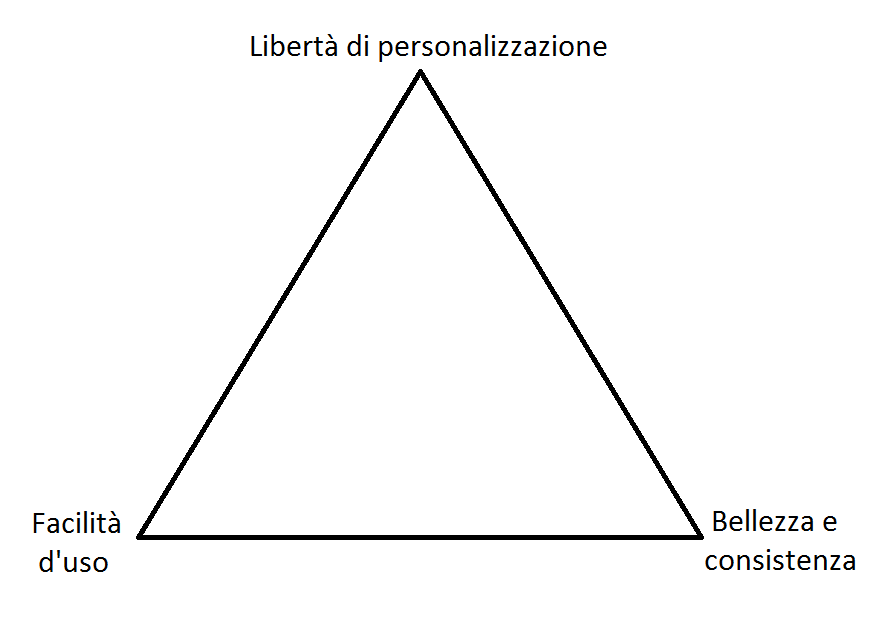
\includegraphics[scale=0.8]{conference_triangle.png}
    	\end{center}
        \caption[Caratteristiche di un tool di personalizzazione di conferenze]{Caratteristiche desiderate in un tool di personalizzazione di conferenze.}
        \label{fig:conference_triangle}
    \end{figure}
    
    In Figura \ref{fig:conference_triangle} vediamo schematizzate le principali caratteristiche che vorremmo uno strumento di personalizzazione di conferenze avesse, che descriviamo qui di seguito:
    
    \begin{itemize}
        \item \textbf{Libertà di personalizzazione}: il tool deve garantire quanta più libertà di personalizzazione, per permettere all'utente di realizzare il più possibile la sua idea di conferenza, adattandola alle sue esigenze e gusti personali;
        \item \textbf{Facilità d'uso}: il tool dev'essere il più facile e intuitivo possibile da utilizzare: è inutile, infatti, mettere l'utente di fronte a una sfilza di bottoni e strumenti se poi l'utente ne utilizzerà soltanto due o tre perché non conosce il significato degli altri;
        \item \textbf{Bellezza e consistenza}: il tool deve favorire la creazione di pagine di conferenze che abbiano uno stile moderno e consistente e, allo stesso tempo, rendere difficile (se non impossibile) la creazione di pagine antiestetiche.
    \end{itemize}
    
    Chiaramente, la situazione ideale sarebbe avere tutte e tre le caratteristiche presenti nel tool di personalizzazione, tuttavia, come vedremo più avanti, non sarà possibile trovare un tool simile e sarà necessario scendere a compromessi.
    
    Prima di iniziare a parlare del tool sviluppato in questa fase del progetto, vediamo prima brevemente qual è la situazione attuale per quanto riguarda la personalizzazione di conferenze in Indico.
    
    \section{Situazione attuale} \label{sec:ccp;situazione_attuale}
    
        La situazione del tool per la personalizzazione di conferenze prima dell'inizio del progetto (e tutt'ora al momento della stesura di questa tesi) era che questo strumento permetteva di creare eventi piuttosto gradevoli e consistenti con lo stile di Indico. Un esempio può essere la conferenza in Figura \ref{fig:conference_old}, della quale possiamo notare lo stile minimale e l'utilizzo di icone consistenti con lo stile di Indico e del \ac{CERN} in generale.
        
        \begin{figure}[h!]
            \begin{center}
        		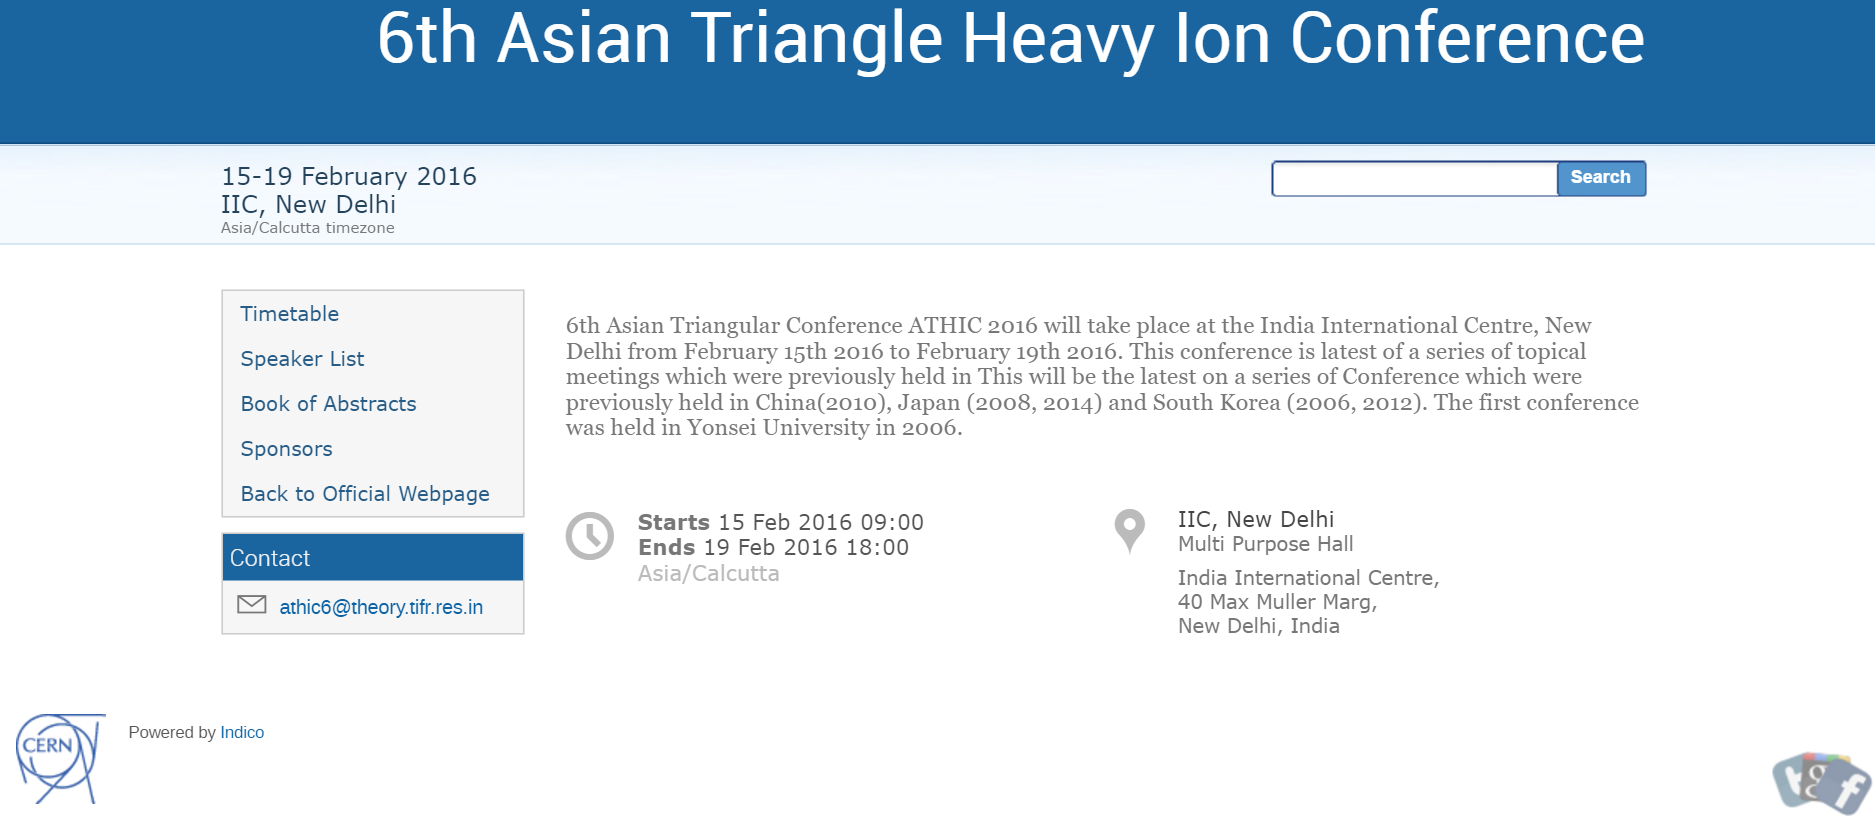
\includegraphics[scale=0.4]{conference_old.png}
        	\end{center}
            \caption[Esempio di conferenza in Indico]{Esempio della situazione attuale delle conferenze in Indico (fonte \url{https://indico.cern.ch/event/487533/}).}
            \label{fig:conference_old}
        \end{figure}
        
        Lo stile, tuttavia, risulta essere non troppo moderno: molte pagine di conferenze su Internet utilizzano elementi dinamici e interattivi ed uno stile, in generale, più moderno.
        
        Per quanto riguarda il tool di personalizzazione vero e proprio, c'è da dire che esso non permette una piena libertà di personalizzazione, mettendo a disposizione dell'utente soltanto pochi stili ed elementi di layout. Inoltre molte opzioni e possono risultare, per l'utente medio, difficili da utilizzare o poco intuitive, anche per il fatto che l'interfaccia non è molto user-friendly, come possiamo vedere in Figura \ref{fig:conference_customization}.
        
        \begin{figure}[h!]
            \begin{center}
        		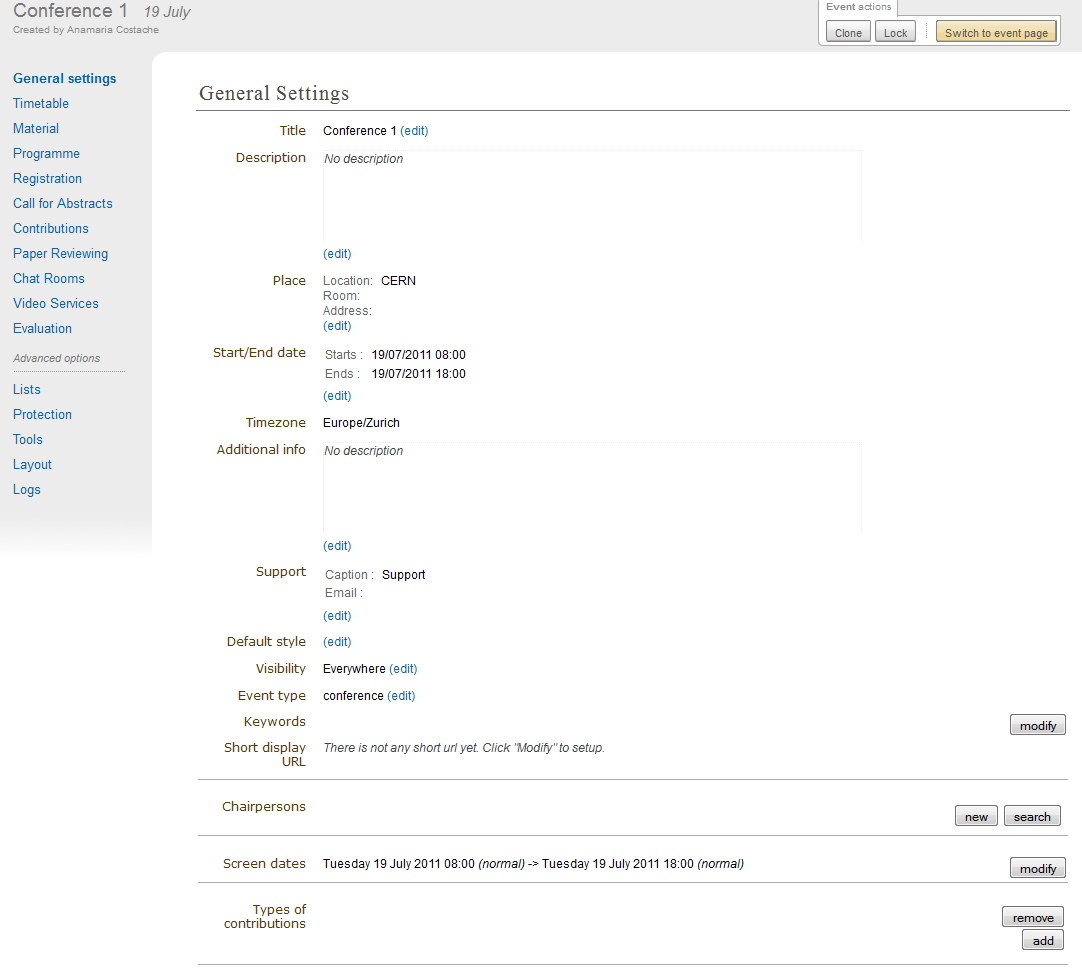
\includegraphics[scale=0.7]{conference_customization.png}
        	\end{center}
            \caption[Tool di configurazione di una conferenza in Indico]{Interfaccia della pagina di configurazione di una conferenza in Indico.}
            \label{fig:conference_customization}
        \end{figure}
        
        Quindi Indico permette di creare pagine di conferenze con stili gradevoli e consistenti, al costo di limitare ampiamente la libertà di personalizzazione, il tutto utilizzando un'interfaccia di personalizzazione non sempre intuitiva.
        
        Tra le opzioni avanzate del tool di personalizzazione, era inoltre presente la possibilità di far caricare all'utente il proprio stile \ac{CSS}. Sfruttando quest'opzione l'utente è in grado di avere pieno controllo sulla personalizzazione della pagina, potendo definire il proprio stile \ac{CSS} in maniera totalmente libera. Tuttavia quest'approccio ha due problemi principali: è complicato da utilizzare, per l'utente medio, e permette all'utente di creare qualsiasi tipo di pagina, comprese pagine brutte, inconsistenti o, in generale, antiestetiche.
        
        \subsection{La necessità di un nuovo strumento} \label{subsec:ccp;sa;necessità_nuovo_strumento}
        
            In questo progetto finale del Progetto KT si è allora cercato di sviluppare un prototipo per un tool di creazione e personalizzazione di conferenze.
            
            Si parla di prototipo in quanto a questa fase sono stati dedicati, da contratto, soltanto gli ultimi mesi del programma di Technical Student a cui ha partecipato il sottoscritto, che sono stati considerati del tutto insufficienti, a priori, per sviluppare un prodotto finito. Inoltre, prima di iniziare lo sviluppo vero e proprio di un tool di personalizzazione di conferenze, era necessario capire in che direzione si voleva portare questo futuro tool, ovvero che forma e caratteristiche dovesse avere. Quest'ultima fase del Progetto KT è stata quindi incentrata proprio su questo: indagare e investigare tutte le possibili soluzioni per un futuro tool di personalizzazione di conferenze sviluppando, a supporto del processo di analisi, un prototipo che rispecchiasse, di volta in volta, le idee proposte.
            
            Questo progetto è stato quindi più un progetto di indagine, riguardo a come strutturare un tool futuro, che di sviluppo. Per questo ci concentreremo, nel seguito della trattazione, su aspetti decisionali e sui vari step che hanno composto questa fase, piuttosto che su aspetti tecnici. Infatti il codice del prototipo sviluppato non verrà utilizzato in alcun modo per lo sviluppo del tool finale, che verrà scritto da zero, probabilmente con i fondi di un secondo Progetto KT per Indico. In ogni caso, il codice del prototipo sviluppato al \ac{CERN} dal sottoscritto negli ultimi mesi è disponibile al seguente repository Github: \url{https://github.com/indico/conference-customization-2.0}.
            
            In generale, i possibili approcci che si potevano intraprendere per la personalizzazione di conferenze erano tre:
            
            \begin{itemize}
                \item \textbf{Approccio alla Facebook}: creare uno stile molto bello, molto carino e consistente ma fornire un solo stile unico uguale per tutti; quest'approccio risulterebbe molto semplice da gestire, ma non fornirebbe alcun tipo di personalizzazione all'utente;
                \item \textbf{Upload di \ac{CSS}}: come l'opzione avanzata già presente in Indico al momento, permettere di caricare i propri stili \ac{CSS} personali permette all'utente di personalizzare la pagina come più gli piace, ma gli da anche la libertà di creare conferenze antiestetiche o inconsistenti (il problema della consistenza è importante in quanto l'organizzazione che gestisce l'istanza di Indico ha una certa immagine da rispettare ed una pagina brutta o con stile diverso si può riflettere negativamente sull'immagine dell'organizzazione);
                \item \textbf{Approccio orientato agli widget}: definire un insieme finito di tipi di widget (come negli smartphone) che l'utente può posizionare nella pagina e personalizzare, entro un certo limite.
            \end{itemize}
            
            Chiaramente le prime due soluzioni rappresentano i due casi estremi in cui si punta tutto alla bellezza e alla consistenza, da un lato, e in cui si punta tutto sulla libertà di personalizzazione, dall'altro. Il terzo approccio è invece un approccio ibrido ed è stata l'opzione che, fin dal principio, è sembrata essere la più promettente e sensata delle tre.
            
            Questa progetto è quindi stato composto da una serie di prove ed errori, idee e suggerimenti, ognuno dei quali veniva proposto all'intero team di Indico durante ogni meeting, che si teneva regolarmente ogni settimana, per decidere se valeva la pena continuare ad investigare in quella direzione o se era necessario un cambio di programma. Spesso infatti il prototipo è stato riscritto quasi da zero. Molte altre volte le modifiche sono invece state minime e graduali, cambiando il prototipo a poco a poco.
            
            Per queste ragioni, nelle Sezioni successive, non mostreremo tutti i singoli passi attraverso i quali il prototipo si è evoluto, ma soltanto i due principali checkpoint dello sviluppo, che rappresentano i due approcci che sono stati principalmente indagati durante questa fase.
            
    \section{Classi di widget} \label{sec:ccp;classi_widget}
    
        Fin da subito l'idea di indagare una soluzione orientata agli widget è piaciuta all'intero team di Indico. Con widget si intendono parti del layout indipendenti, riusabili e componibili. Il primo obiettivo è stato quindi definire, a grandi linee, le classi di widget che si volevano includere nel tool di personalizzazione e, per ognuna di esse, dare un'idea generale di come si poteva personalizzare e come avrebbe dovuto comportarsi.
        
        Alcuni widget avrebbero ripreso la funzione di alcune parti della vecchia pagina delle conferenze presente in Indico, come ad esempio si è pensato subito ad un widget per mostrare la timetable della conferenza, o ancora un widget che visualizzasse il luogo dell'evento. Altri widget invece sono stati ideati sul momento, tramite i suggerimenti di tutti i membri del team e attraverso svariate sessioni di brainstorming.
        
        Di seguito proponiamo la lista delle classi di widget ideate durante questa fase, con tanto di descrizione. Le classi di widget proposte sono state suddivise in due classi: widget generici, che possono essere usati per molti fini diversi tra loro ed il cui utilizzo dipende dall'utente, e widget dedicati, che invece sono più specializzati ed hanno uno scopo ben preciso. Nelle Figure dalla \ref{fig:list} alla \ref{fig:menu_vertical} possiamo vedere alcuni degli sketch disegnati dal sottoscritto durante le prime fasi di brainstorming con l'intero team per avere meglio un'idea di come sarebbero apparsi, graficamente, i vari widget, in modo da strutturare la pagina in modo adeguato.
        
        \begin{itemize}
            \item Widget generici
                \begin{itemize}
                    \item \textbf{Lista}: una generica lista di elementi testuali, come una frase, una descrizione o informazioni utili (Figura \ref{fig:list} lo stile prevedeva la scelta del bordo (con o senza), la possibilità di aggiungere un titolo e la possibilità di formattare il testo, ad esempio inserendo elenchi puntati o icone;
                    \item \textbf{Carosello}: una serie di elementi grafici o testuali che si alternano, scorrendo orizzontalmente; la scelta dello stile includeva la selezione di un'immagine di sfondo, la possibilità di visualizzare un elemento alla volta (Figura \ref{fig:carousel_single-element}) o più di uno (Figura \ref{fig:carousel_multi-element}), l'aggiunta di un titolo, la possibilità di mostrare o meno una breve descrizione sotto ogni elemento e la possibilità di avere delle frecce o bottoni di navigazione; questo tipo di widget può essere utilizzato per mostrare gli argomenti principali di una conferenza, o i principali sponsor, o semplicemente come galleria fotografica;
                    \item \textbf{Riquadro}: un widget generico (Figura \ref{fig:box}) che può contenere elementi testuali, grafici o una combinazione dei due, ad esempio utilizzandolo come titolo per una conferenza o per mostrare avvisi importanti; lo stile prevede la scelta del bordo e del titolo, nonché del contenuto.
                \end{itemize}
            \item Widget dedicati
                \begin{itemize}
                    \item \textbf{Date}: widget che mostra le date principali dell'evento; lo stile può essere sotto forma di lista o di carosello; l'idea era di poter caricare le date di inizio e fine dell'evento direttamente dal database di Indico e allo stesso tempo dare la possibilità all'utente di aggiungere dare aggiuntive;
                    \item \textbf{Luogo}: widget che mostra il luogo fisico in cui si tiene la conferenza; lo stile prevede una mappa (tramite le \ac{API} di Google Maps o tramite immagine, come in Figura \ref{fig:map}), un indirizzo, delle indicazioni stradali oppure una combinazione delle tre cose (Figura \ref{fig:map_address_directions}); come prima, l'idea era di caricare il luogo direttamente da Indico ed eventualmente aggiungere mappe extra;
                    \item \textbf{Materiale}: widget per visualizzare tutto il materiale caricato nella pagina dell'evento; lo stile può essere sia lista che carosello; l'idea era di caricare i file presenti dal database ed eventualmente associare ad ognuno di essi un'azione (apri/scarica/ecc\dots);
                    \item \textbf{Persone coinvolte}: un elenco di persone coinvolte nella conferenza (ad esempio autori o speaker) sotto forma di lista o carosello;
                    \item \textbf{Condivisione su social media}: una serie di bottoni per condividere in modo rapido la pagina dell'evento tramite i principali social media, come Facebook, Twitter o Google+; il widget è stato pensato in versione sia orizzontale (Figura \ref{fig:share_horizontal}) che verticale (Figura \ref{fig:share_vertical}) e con la possibilità di aggiungere accanto ad ogni bottone il numero di condivisioni tramite quel particolare social media;
                    \item \textbf{Notizie tramite social media}: ultime notizie caricate dalla pagina relativa alla conferenza su un particolare social media (Figura \ref{fig:social_media_news}); in questo caso l'utente dovrebbe specificare da quale account/pagina caricare le notizie da visualizzare;
                    \item \textbf{Menu}: semplice menu, orizzontale (Figura \ref{fig:menu_horizontal}) o verticale (Figura \ref{fig:menu_vertical}), con bottoni e la possibilità di aggiungere sotto-menu innestati;
                    \item \textbf{Titolo}: un widget orizzontale, largo quanto tutta la pagina, contenente il titolo della conferenza e uno sfondo scelto dall'utente;
                    \item \textbf{Ricerca}: barra di ricerca di Indico o di Google;
                    \item \textbf{Timetable}: widget dedicato alla timetable della conferenza.
                \end{itemize}
        \end{itemize}
        
       	\begin{figure}[h!]
       		\begin{center}
       			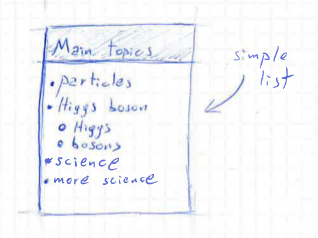
\includegraphics[scale=0.6]{list.png}
       		\end{center}
       		\caption[Sketch del widget ``lista'']{Sketch del widget ``lista''.}
       		\label{fig:list}
       	\end{figure}
       	
       	\begin{figure}[h!]
       		\begin{center}
       			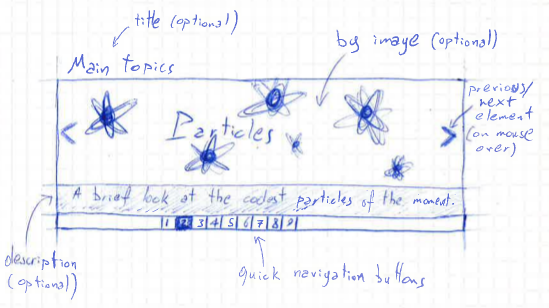
\includegraphics[scale=0.5]{carousel_single-element.png}
       		\end{center}
       		\caption[Sketch del widget ``carosello'' (elemento singolo)]{Sketch del widget ``carosello'' con un solo elemento a volta.}
       		\label{fig:carousel_single-element}
       	\end{figure}
        
       	\begin{figure}[h!]
       		\begin{center}
       			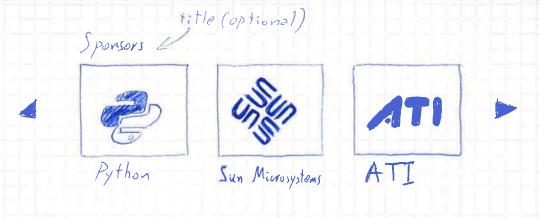
\includegraphics[scale=0.6]{carousel_multi-element.png}
       		\end{center}
       		\caption[Sketch del widget ``carosello'' (elementi multipli)]{Sketch del widget ``carosello'' con più elementi a volta.}
       		\label{fig:carousel_multi-element}
       	\end{figure}
        
       	\begin{figure}[h!]
       		\begin{center}
       			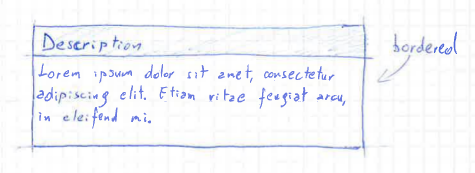
\includegraphics[scale=0.6]{box.png}
       		\end{center}
       		\caption[Sketch del widget ``riquadro'']{Sketch del widget ``riquadro''.}
       		\label{fig:box}
       	\end{figure}
       	
       	\begin{figure}[h!]
       		\begin{center}
       			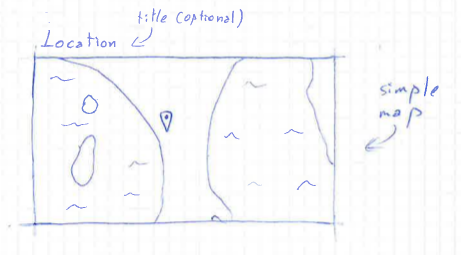
\includegraphics[scale=0.6]{map.png}
       		\end{center}
       		\caption[Sketch del widget ``luogo'' (semplice)]{Sketch del widget ``luogo'' con la sola mappa.}
       		\label{fig:map}
       	\end{figure}
       	
       	\begin{figure}[h!]
       		\begin{center}
       			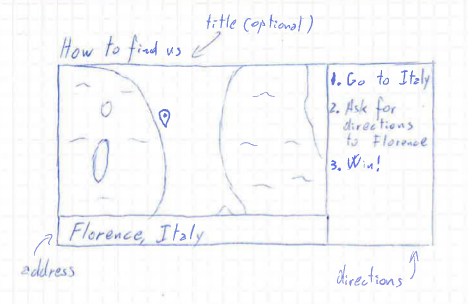
\includegraphics[scale=0.6]{map_address_directions.png}
       		\end{center}
       		\caption[Sketch del widget ``luogo'' (con indirizzo e indicazioni)]{Sketch del widget ``luogo'' con mappa, indirizzo e indicazioni stradali.}
       		\label{fig:map_address_directions}
       	\end{figure}
       	
       	\begin{figure}[h!]
       		\begin{center}
       			
\includegraphics[scale=0.6]{share_horizontal.png}
       		\end{center}
       		\caption[Sketch del widget ``condivisione su social media'' (orizzontale)]{Sketch del widget ``condivisione su social media'' in formato orizzontale.}
       		\label{fig:share_horizontal}
       	\end{figure}
       	
       	\begin{figure}[h!]
       		\begin{center}
       			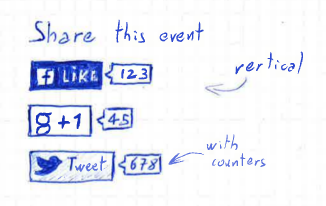
\includegraphics[scale=0.6]{share_vertical.png}
       		\end{center}
       		\caption[Sketch del widget ``condivisione su social media'' (verticale)]{Sketch del widget ``condivisione su social media'' in formato verticale.}
       		\label{fig:share_vertical}
       	\end{figure}
       	
       	\begin{figure}[h!]
       		\begin{center}
       			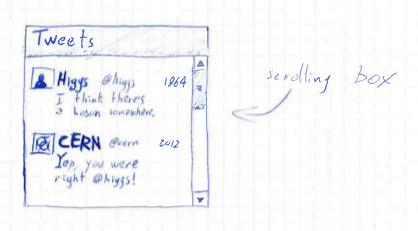
\includegraphics[scale=0.6]{social_media_news.png}
       		\end{center}
       		\caption[Sketch del widget ``notizie tramite social media'']{Sketch del widget ``notizie tramite social media''.}
       		\label{fig:social_media_news}
       	\end{figure}
       	
       	\begin{figure}[h!]
       		\begin{center}
       			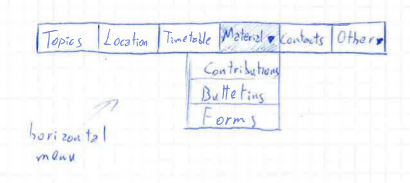
\includegraphics[scale=0.6]{menu_horizontal.png}
       		\end{center}
       		\caption[Sketch del widget ``menu'' (orizzontale)]{Sketch del widget ``menu'' in formato orizzontale.}
       		\label{fig:menu_horizontal}
       	\end{figure}
       	
       	\begin{figure}[h!]
       		\begin{center}
       			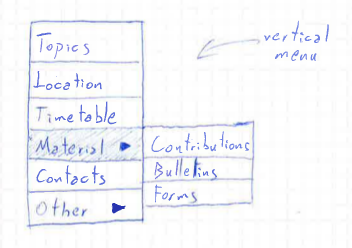
\includegraphics[scale=0.6]{menu_vertical.png}
       		\end{center}
       		\caption[Sketch del widget ``menu'' (verticale)]{Sketch del widget ``menu'' in formato verticale.}
       		\label{fig:menu_vertical}
       	\end{figure}
       	
       	\FloatBarrier
       	
    \section{User Interface} \label{sec:ccp;user_interface}
    
        Durante le prime fasi di brainstorming al \ac{CERN} si sono anche definiti alcuni elementi base dell'interfaccia utente che si volevano includere nella versione finale del progetto.
        
        L'idea era quella di progettare uno strumento di personalizzazione di conferenze che fosse facile e intuitivo da usare. Rimanendo sulla scia di idee degli widget, uno dei concetti chiave che sono emersi è stata la possibilità di avere un'interfaccia basata sul drag-and-drop, ovvero poter piazzare gli widget all'interno della pagina semplicemente trascinandoli col mouse e, in generale, poterli personalizzare tramite pochi click. Si era infatti pensato anche che, in fase di personalizzazione della pagina, sopra ogni widget sarebbe potuta comparire una serie di bottoni per la modifica e personalizzazione dello widget, in modo da mantenere ogni widget graficamente separato dall'altro (anche in fase di modifica) e di rendere l'intero processo il più intuitivo possibile.
       	
    \section{Approccio a widget totale} \label{sec:ccp;approccio_widget_totale}
    
        Una volta definite le classi di widget da includere, ovvero i ``mattoni'' elementari che avrebbero composto la pagina delle conferenze, si è iniziato a pensare a come strutturare la pagina di una conferenza, ovvero come gestire questi widget.
        
        Il primo approccio perseguito prevedeva una struttura della pagina successivamente denominata \textit{full widget-based layout}, ovvero ``struttura totalmente orientata agli widget''. Questo approccio prevedeva di rappresentare la pagina delle conferenze tramite un'enorme griglia che dividesse la pagina in tanti spazi vuoti: in ognuno di questi spazi l'utente avrebbe potuto piazzare un widget ed eventualmente ridimensionarlo a piacimento in modo da fargli occupare più spazi. La suddivisione orizzontale starebbe stata fissa, mentre gli spazi sarebbero potuti estendersi all'infinito in senso verticale. Inoltre erano stati ideati dei contenitori, con lo scopo di poter raggruppare al loro interno widget o altri contenitori.
        
        In Figura \ref{fig:full_widget_layout} vediamo lo sketch fatto dal sottoscritto durante lo studio di questo approccio, per poter essere presentato al resto del team.
        
       	\begin{figure}[h!]
       		\begin{center}
       			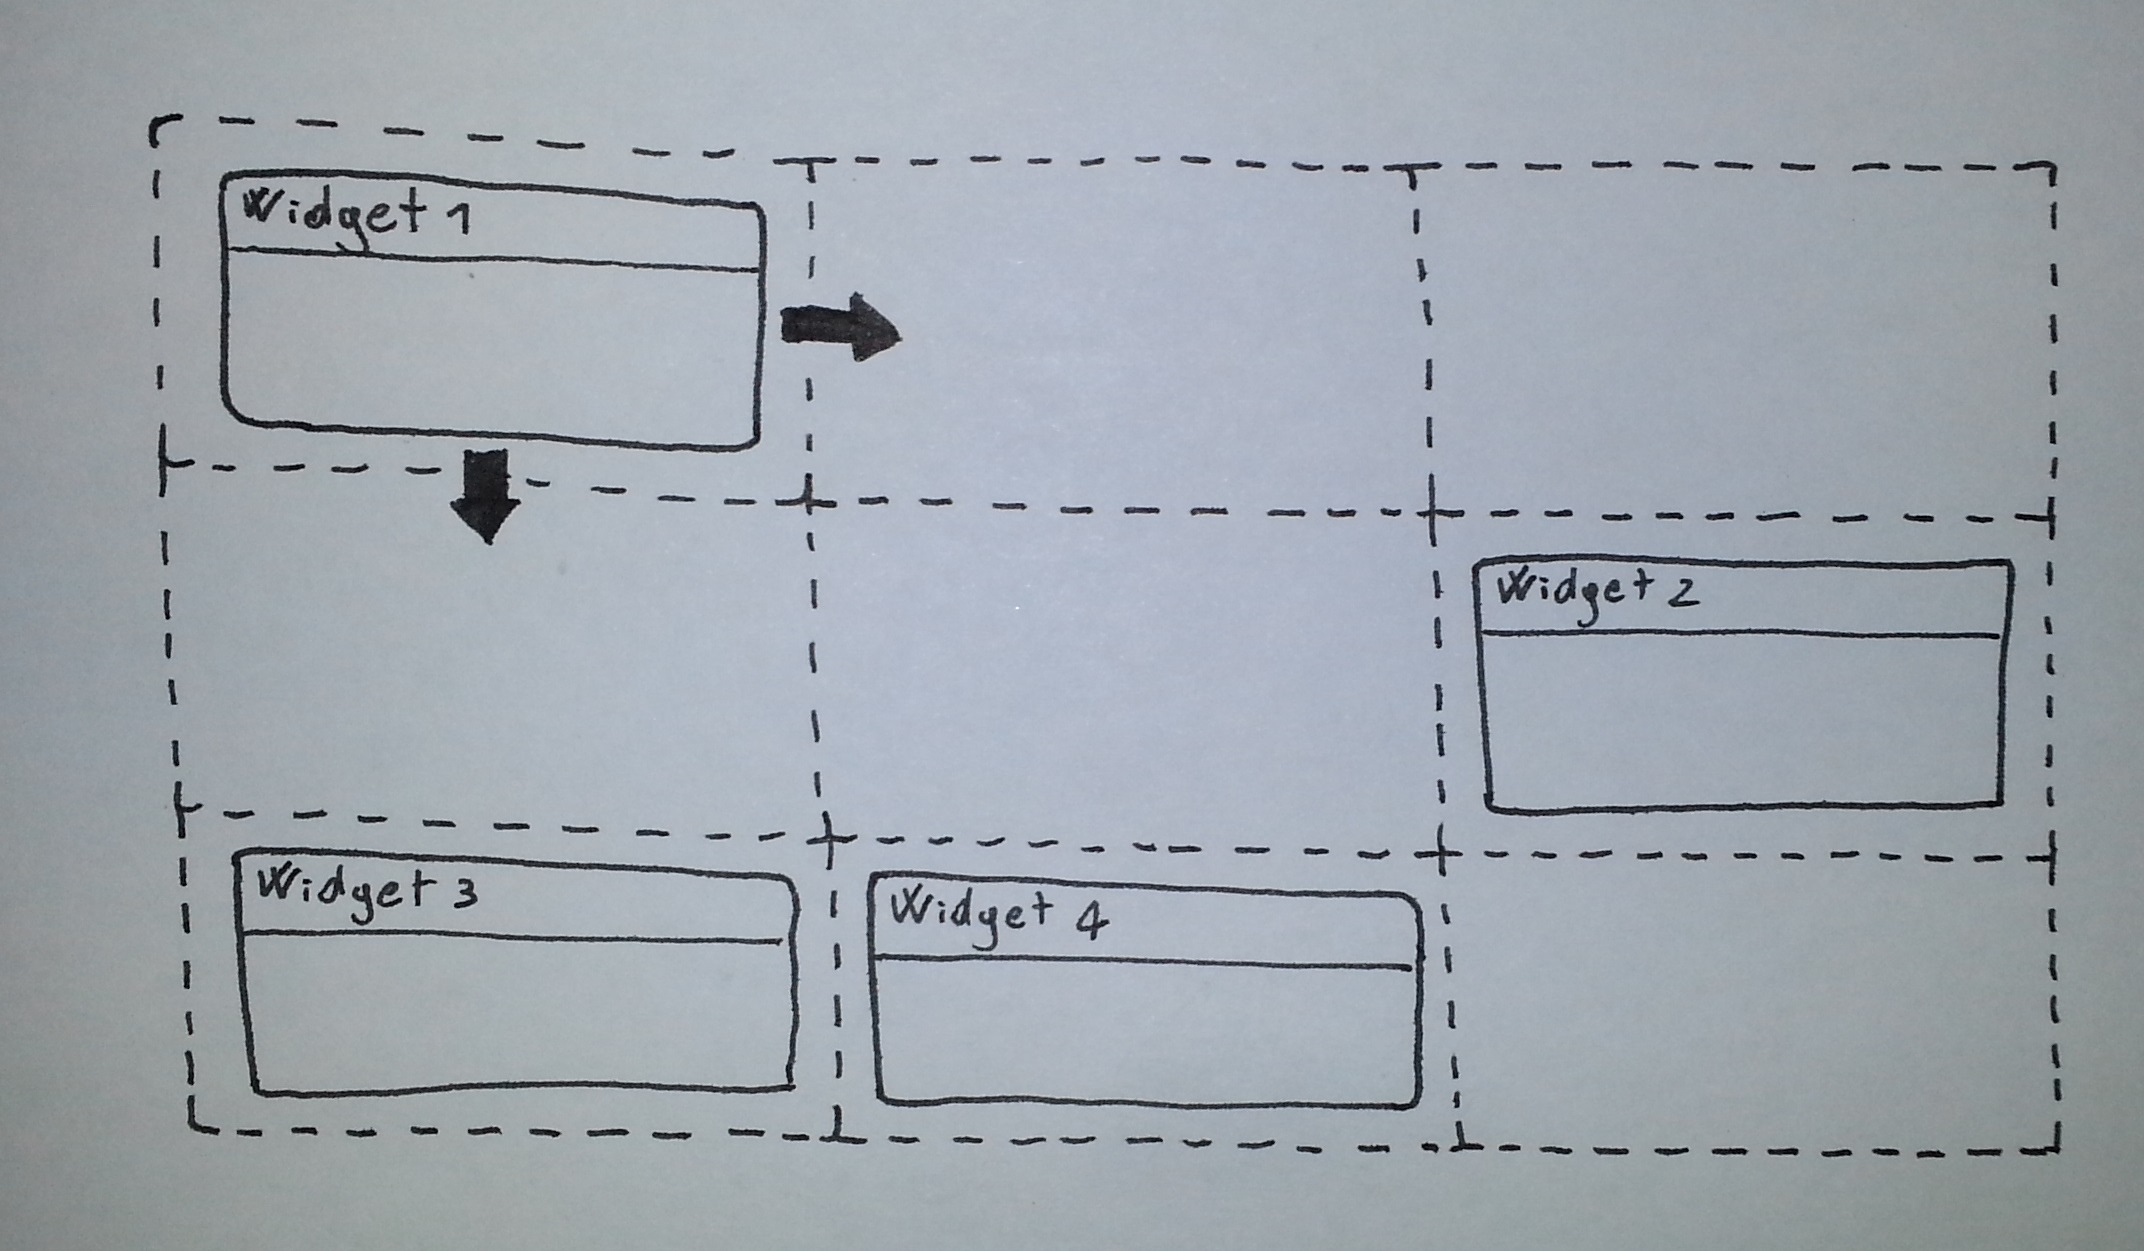
\includegraphics[scale=0.15]{full_widget_layout.jpg}
       		\end{center}
       		\caption[Sketch della struttura a widget totale]{Sketch del funzionamento della struttura totalmente orientata agli widget.}
       		\label{fig:full_widget_layout}
       	\end{figure}
       	
       	L'idea di poter creare uno strumento orientato agli widget e dotato di interfaccia drag-and-drop ha tuttavia fatto perdere di vista il fatto che, con una struttura del genere, veniva data all'utente troppa libertà di personalizzazione, forse in grado anche peggiore rispetto all'upload dello stile \ac{CSS} (come avviene attualmente in Indico). Infatti con questa struttura era possibile creare pagine molto brutte e instabili, ad esempio creando widget giganteschi che occupassero tutta la pagina, o creando serie di contenitori innestati, rendendo illeggibile il contenuto. Inoltre anche solo il fatto di poter piazzare gli widget ovunque l'utente desiderasse incoraggiava la creazione di pagine inconsistenti e senza un ordine logico preciso.
       	
       	Il problema di questo approccio era quindi che, nonostante si utilizzassero un'interfaccia drag-and-drop e elementi basati su widget per rendere lo stile più moderno, l'utente aveva ancora troppa libertà di personalizzazione, rischiando di creare pagine altamente antiestetiche e inutilizzabili.
    
    \section{Approccio a widget ibrido} \label{sec:ccp;approccio_widget_ibrido}
    
        Dopo molte sessioni di brainstorming, durante le quali sono state fatte molte proposte per risolvere il problema della struttura totalmente orientata agli widget, e dopo molte modifiche al prototipo, si è raggiunto un consenso con la struttura detta \textit{block-widget hybrid layout}, ovvero ``struttura ibrida basata su blocchi e widget''.
        
        L'idea di base di questo approccio è di suddividere la pagina verticalmente in sezioni, che occupano l'intera larghezza della pagina. Ognuna di queste sezioni è detta \textit{blocco} e rappresenta una sezione della pagina dove viene definito un unico stile di formattazione. All'interno del blocco possono essere messi degli widget, ordinandoli orizzontalmente o verticalmente, a seconda del blocco scelto.
        
       	\begin{figure}[h!]
       		\begin{center}
       			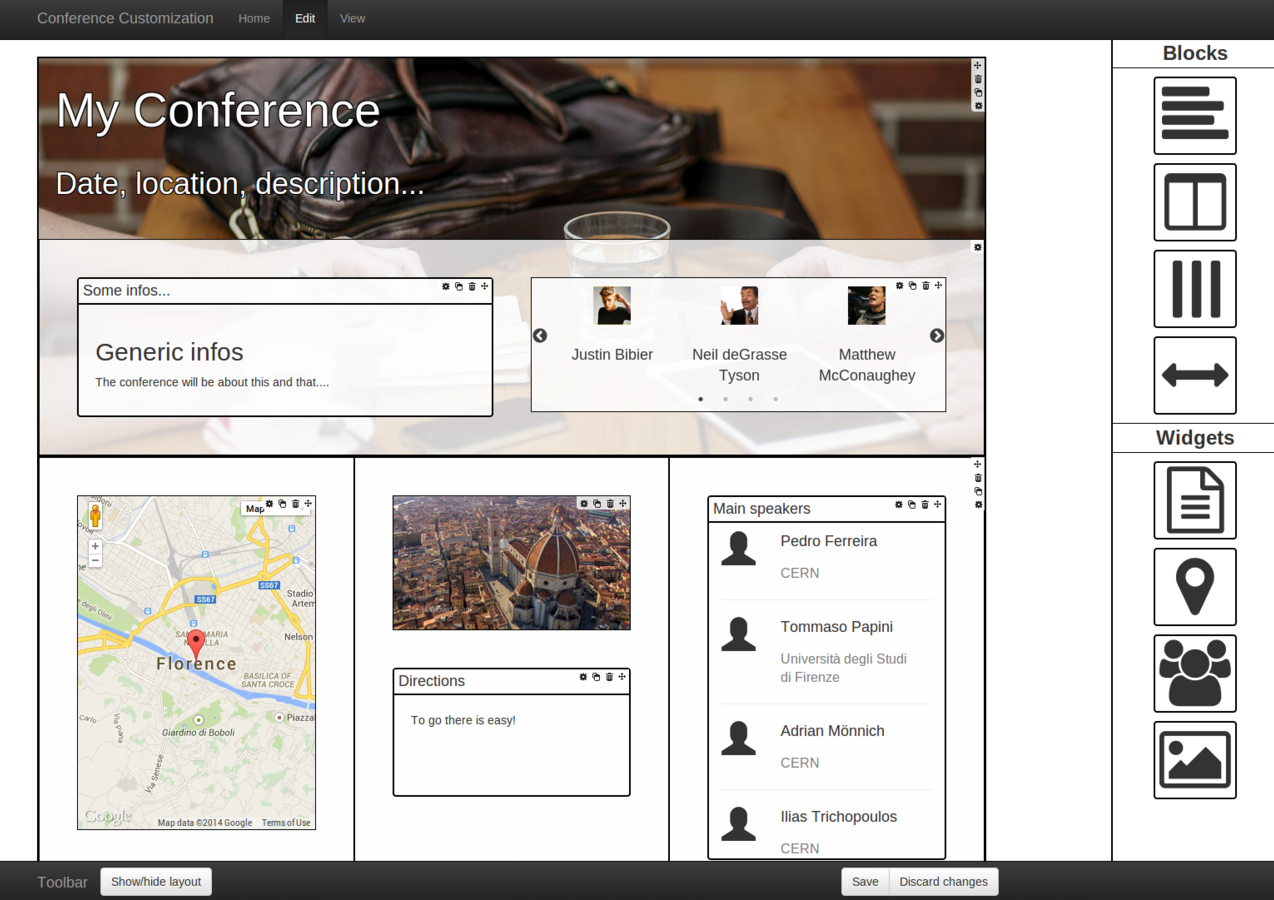
\includegraphics[scale=0.5]{prototype.png}
       		\end{center}
       		\caption[Versione finale del prototipo]{Schermata d'esempio della versione finale del prototipo.}
       		\label{fig:prototype}
       	\end{figure}
       	
       	In Figura \ref{fig:prototype} vediamo una schermata rappresentativa del prototipo costruito seguendo la struttura di quest'ultimo approccio, ovvero una struttura ibrida con widget e blocchi. Sulla destra possiamo vedere una barra contenente i blocchi e gli widget implementati. I blocchi disponibili sono: colonna singola, due colonne, tre colonne o blocco orizzontale. Gli widget invece sono: riquadro testuale, luogo (con mappa tramite Google Maps), persone coinvolte o immagine. Per ogni widget e per ogni blocco possiamo notare, nell'angolo in alto a destra, quattro icone che servono, intuitivamente, per personalizzare, duplicare, eliminare o trascinare quel widget o blocco. Tutta l'interfaccia del prototipo in quest'ultima fase supportava pienamente il drag-and-drop e, cliccando sul pulsante per la personalizzazione di un widget/blocco, si apriva un riquadro popup sullo schermo con i campi relativi a quell'elemento che l'utente può modificare.
       	
       	Tirando le conclusioni, quest'ultimo approccio combina la facilità di utilizzo (tramite interfaccia drag-and-drop) con uno stile moderno e gradevole (grazie a blocchi e widget), il tutto permettendo all'utente di personalizzare i vari elementi della pagina e modellare la conferenza a proprio piacimento, entro certi limiti. Ovviamente con questo approccio non si ha più la totale libertà di personalizzazione, tuttavia si è giunti alla conclusione che di fatto, all'utente, non serve avere totale libertà, fin tanto che lo strumento che sta utilizzando gli permette di creare pagine belle e che rispecchino la sua idea di conferenza. Questo approccio ibrido è quindi risultato, alla fine dei conti, il più solido e ben strutturato e, anche se il codice scritto per il prototipo non verrà riutilizzato, i risultati ottenuti con questa fase d'indagine saranno sicuramente essenziali per lo sviluppo dello strumento di personalizzazione delle conferenze vero e proprio.

		\chapter{Altri progetti} \label{chap:altri_progetti}

    In quest'ultimo Capitolo riguardante il Progetto KT, illustriamo alcuni progetti minori che hanno fatto parte del Progetto KT e del programma di Techical Student in generale.

    \section{Chiusura dei ticket} \label{sec:ap;chiusura_ticket}
    
        Come accennato all'interno del Capitolo \ref{chap:indico}, Indico è un software open source in continuo sviluppo. Ogni problema da risolvere o funzionalità da aggiungere viene gestita tramite un sistema di ticket. Un ticket rappresenta, appunto, un qualche problema di Indico, da risolvere per garantire il corretto funzionamento dell'applicazione, oppure una funzionalità che gli utenti gradirebbero avere in Indico. Una volta che è stato scritto dagli sviluppatori il codice necessario a risolvere il problema espresso da un ticket, allora si dice che il ticket è stato ``chiuso''.
        
        Durante il periodo di Techical Student, il sottoscritto si è trovato a dover chiudere alcuni ticket di svariata natura. I primi ticket sono stati chiusi durante le prime settimane di lavoro nel team di Indico, con lo scopo di familiarizzare col programma ed il suo codice. Altri ticket sono invece stati chiusi durante tempi morti del periodo lavorativo.
        
        Alcuni tipi ti ticket chiusi includono:
        
        \begin{itemize}
            \item permettere di fare una ricerca degli utenti senza considerare gli accenti (ad esempio cercare ``Gonzales'' deve ritornare come risultato anche cognomi come ``Gonzáles'');
            \item aggiungere un link diretto alla visualizzazione dettagliata nella timetable;
            \item mostrare la disponibilità delle stanze quando si crea o modifica un meeting.
        \end{itemize}
    
    \section{Nuova pagina delle statistiche} \label{sec:ap;nuova_pagina_statistiche}
    
        Per prendere dimestichezza con la libreria jqPlot, per la rappresentazione di grafici, prima di intraprendere il progetto di Instance Tracking (Capitolo \ref{chap:instance_tracker}) si è aggiornata la pagina delle statistiche presente in Indico. Per ogni categoria di Indico è infatti presente una pagina delle statistiche che mostra, per quella determinata categoria, una serie di statistiche come numero di eventi o numero di file aggiunti nel tempo.
        
        Dato che lo stile della pagina era piuttosto datato e poco moderno, si è deciso di migliorare la pagina, sfruttando la libreria jqPlot, rinnovandone lo stile. Il risultato si può vedere in Figura \ref{fig:category_statistics}.
        
       	\begin{figure}[h!]
       		\begin{center}
       			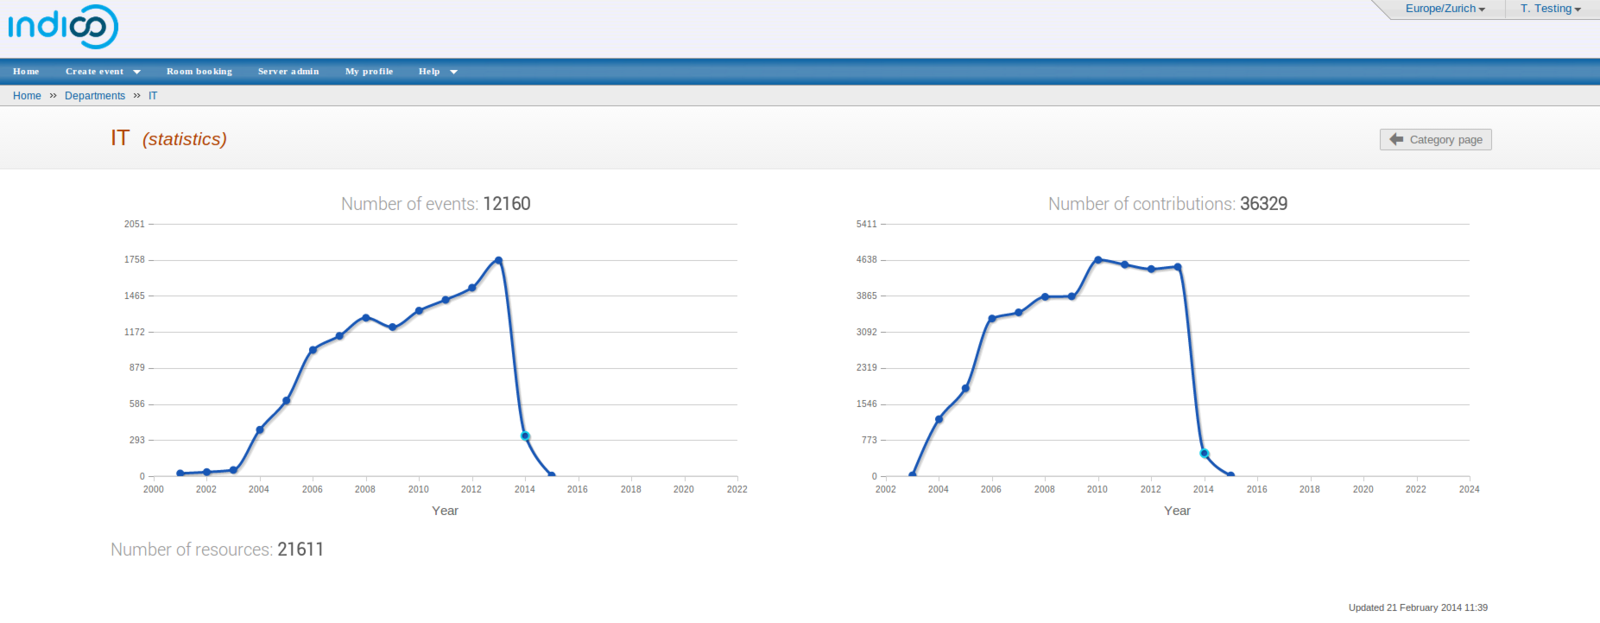
\includegraphics[scale=0.23]{category_statistics.png}
       		\end{center}
       		\caption[Statistiche di una categoria]{Nuova pagina delle statistiche di una categoria in Indico.}
       		\label{fig:category_statistics}
       	\end{figure}

    \section{Installazione su Windows Server} \label{sec:ap;installazione_windows_server}
    
        Uno degli obiettivi del KT Project per Indico includeva l'esplorazione di possibilità per un possibile adattamento di Indico a sistemi Windows Server. Indico infatti è stato progettato per poter essere installato su sistemi Unix e non supporta sistemi Windows. Nell'ottica del Progetto KT, si è tuttavia pensato che molte aziende o organizzazioni potrebbero aver già un server in utilizzo con installato Windows Server. Queste organizzazioni potrebbero essere scoraggiate dall'utilizzare Indico, per il quale dovrebbero installare un secondo server con sistema Unix.
        
        I problemi principali dell'installazione di Indico su Windows Server erano principalmente due: riuscire a installare in ambiente Windows tutte le librerie necessarie a Indico e riuscire a far funzionare \ac{WSGI} col web server messo a disposizione da Windows, \acr{IIS}.
        
        Il problema relativo alle librerie era dovuto al fatto che non tutte le librerie utilizzate da Indico erano state distribuite per Windows. Dopo circa un mese di ricerca, si sono riuscite a trovare su Internet, da fonti ufficiali o meno, tutte le librerie necessarie. Alcune di queste librerie si sono trovate in formato \bash{.exe}, che rappresentava la situazione ottima in quanto le più semplici da installare su Windows. Il resto (la maggior parte) sono state installate da Python egg (\bash{.egg}) o da tarball (\bash{.tar.gz}).
        
        Il problema relativo a \ac{WSGI} stava invece nel riuscire a trovare, installare e configurare un wrapper funzionante per \ac{IIS}. \ac{WSGI} è un'interfaccia che permette la comunicazione tra applicazioni Python e un determinato web server. Per poter far funzionare \ac{WSGI} con un determinato web server, è tuttavia necessario trovare un wrapper adatto, come ad esempio \bash{mod_wsgi} per Apache. Per trovare un wrapper adatto si sono provate diverse soluzioni, come WFastCGI, isapi-wsgi o PyISAPIe (si veda \cite{wiki:wsgi}), ma non sono risultate sufficienti. Si è invece riusciti a far comunicare correttamente \ac{WSGI} con \ac{IIS} tramite un pacchetto sviluppato dalla società HeliconTech e scaricabile al seguente indirizzo: \url{http://www.helicontech.com/zoo/gallery/PythonHostingPackage.html}.
        
        Dopo aver risolto questi due problemi, si era riusciti ad avviare Indico e ad eseguire alcune semplici azioni con esso. Tuttavia Indico presentava ancora seri problemi, come immagini mancanti o alcune librerie non pienamente funzionanti. A questo punto, però, si è deciso di lasciar perdere questo progetto e di dichiarare fallimentare l'installazione di Indico su Windows Server. In fin dei conti, l'installazione su Windows Server rimaneva un progetto minore del KT Project e, al momento, stava già facendo perdere troppo tempo, che sarebbe stato meglio speso su altri progetti più importanti, come l'Instance Tracking.

	
	\part{Note e conclusioni} \label{part:note_conclusioni}
		\chapter{Conclusioni} \label{chap:conclusioni}


		
%********************************************************************
% Back matter
%********************************************************************
	
	%********************************************************************
% Bibliography
%********************************************************************

\cleardoublepage

\manualmark
\markboth{\spacedlowsmallcaps{\bibname}}{\spacedlowsmallcaps{\bibname}} 

\refstepcounter{dummy}
\addtocontents{toc}{\protect\vspace{\beforebibskip}}
\addcontentsline{toc}{chapter}{\tocEntry{\bibname}}

\nocite{*}
\bibliographystyle{plainnat}
\label{app:bibliography} 
\bibliography{back/bibliography}


\end{document}
        \makeatother

\end{document}
